% Options for packages loaded elsewhere
\PassOptionsToPackage{unicode}{hyperref}
\PassOptionsToPackage{hyphens}{url}
%
\documentclass[
]{book}
\usepackage{lmodern}
\usepackage{amssymb,amsmath}
\usepackage{ifxetex,ifluatex}
\ifnum 0\ifxetex 1\fi\ifluatex 1\fi=0 % if pdftex
  \usepackage[T1]{fontenc}
  \usepackage[utf8]{inputenc}
  \usepackage{textcomp} % provide euro and other symbols
\else % if luatex or xetex
  \usepackage{unicode-math}
  \defaultfontfeatures{Scale=MatchLowercase}
  \defaultfontfeatures[\rmfamily]{Ligatures=TeX,Scale=1}
\fi
% Use upquote if available, for straight quotes in verbatim environments
\IfFileExists{upquote.sty}{\usepackage{upquote}}{}
\IfFileExists{microtype.sty}{% use microtype if available
  \usepackage[]{microtype}
  \UseMicrotypeSet[protrusion]{basicmath} % disable protrusion for tt fonts
}{}
\makeatletter
\@ifundefined{KOMAClassName}{% if non-KOMA class
  \IfFileExists{parskip.sty}{%
    \usepackage{parskip}
  }{% else
    \setlength{\parindent}{0pt}
    \setlength{\parskip}{6pt plus 2pt minus 1pt}}
}{% if KOMA class
  \KOMAoptions{parskip=half}}
\makeatother
\usepackage{xcolor}
\IfFileExists{xurl.sty}{\usepackage{xurl}}{} % add URL line breaks if available
\IfFileExists{bookmark.sty}{\usepackage{bookmark}}{\usepackage{hyperref}}
\hypersetup{
  pdftitle={衛星BASIC},
  pdfauthor={Tamaki.M},
  hidelinks,
  pdfcreator={LaTeX via pandoc}}
\urlstyle{same} % disable monospaced font for URLs
\usepackage{longtable,booktabs}
% Correct order of tables after \paragraph or \subparagraph
\usepackage{etoolbox}
\makeatletter
\patchcmd\longtable{\par}{\if@noskipsec\mbox{}\fi\par}{}{}
\makeatother
% Allow footnotes in longtable head/foot
\IfFileExists{footnotehyper.sty}{\usepackage{footnotehyper}}{\usepackage{footnote}}
\makesavenoteenv{longtable}
\usepackage{graphicx,grffile}
\makeatletter
\def\maxwidth{\ifdim\Gin@nat@width>\linewidth\linewidth\else\Gin@nat@width\fi}
\def\maxheight{\ifdim\Gin@nat@height>\textheight\textheight\else\Gin@nat@height\fi}
\makeatother
% Scale images if necessary, so that they will not overflow the page
% margins by default, and it is still possible to overwrite the defaults
% using explicit options in \includegraphics[width, height, ...]{}
\setkeys{Gin}{width=\maxwidth,height=\maxheight,keepaspectratio}
% Set default figure placement to htbp
\makeatletter
\def\fps@figure{htbp}
\makeatother
\setlength{\emergencystretch}{3em} % prevent overfull lines
\providecommand{\tightlist}{%
  \setlength{\itemsep}{0pt}\setlength{\parskip}{0pt}}
\setcounter{secnumdepth}{5}
\usepackage{booktabs}
\usepackage[]{natbib}
\bibliographystyle{apalike}

\title{衛星BASIC}
\author{Tamaki.M}
\date{2020-11-05}

\begin{document}
\maketitle

{
\setcounter{tocdepth}{1}
\tableofcontents
}
\hypertarget{ux521dux3081ux306b}{%
\chapter*{初めに}\label{ux521dux3081ux306b}}
\addcontentsline{toc}{chapter}{初めに}

\hypertarget{ux306aux305cux4ecaux30eaux30e2ux30fcux30c8ux30bbux30f3ux30b7ux30f3ux30b0ux304cux6ce8ux76eeux3092ux96c6ux3081ux3066ux3044ux308bux306eux304b}{%
\section{なぜ今、リモートセンシングが注目を集めているのか}\label{ux306aux305cux4ecaux30eaux30e2ux30fcux30c8ux30bbux30f3ux30b7ux30f3ux30b0ux304cux6ce8ux76eeux3092ux96c6ux3081ux3066ux3044ux308bux306eux304b}}

\hypertarget{ux30eaux30e2ux30fcux30c8ux30bbux30f3ux30b7ux30f3ux30b0ux30c7ux30fcux30bfux6d3bux7528ux4e8bux4f8b}{%
\section{リモートセンシングデータ活用事例}\label{ux30eaux30e2ux30fcux30c8ux30bbux30f3ux30b7ux30f3ux30b0ux30c7ux30fcux30bfux6d3bux7528ux4e8bux4f8b}}

\hypertarget{ux4f5cux696dux74b0ux5883}{%
\section{作業環境}\label{ux4f5cux696dux74b0ux5883}}

2020年10月現在\\
Windows 10 64bit\\
QGIS 3.14.16

\hypertarget{ux4e8bux524dux6e96ux5099}{%
\chapter{事前準備}\label{ux4e8bux524dux6e96ux5099}}

\hypertarget{ux885bux661fux30c7ux30fcux30bfux306eux7a2eux985e}{%
\section{衛星データの種類}\label{ux885bux661fux30c7ux30fcux30bfux306eux7a2eux985e}}

\hypertarget{ux885bux661fux30c7ux30fcux30bfux3092ux30c0ux30a6ux30f3ux30edux30fcux30c9ux3067ux304dux308bux30b5ux30a4ux30c8}{%
\section{衛星データをダウンロードできるサイト}\label{ux885bux661fux30c7ux30fcux30bfux3092ux30c0ux30a6ux30f3ux30edux30fcux30c9ux3067ux304dux308bux30b5ux30a4ux30c8}}

\begin{itemize}
\item
  USGS EarthExplorer\\
  (\url{https://earthexplorer.usgs.gov/})\\
  アメリカ地質調査所(USGS)が衛星画像データを無償で提供しているサイト  
\item
  EO Browser
  (\url{https://www.sentinel-hub.com/explore/eobrowser/})\\
  Sinergiseが衛星データを無償で提供しているサイト。ブラウザ上で、解析や計測を行うことも可能。
\item
  LAADS DAAC
  (\url{https://ladsweb.modaps.eosdis.nasa.gov/})
  NASAが衛星データを無償提供しているサイト。
\item
  Google earth engine
  (\url{https://earthengine.google.com/})
\end{itemize}

\hypertarget{ux885bux661fux30c7ux30fcux30bfux306eux53d6ux5f97ux65b9ux6cd5usgsux7de8}{%
\chapter{衛星データの取得方法(USGS編)}\label{ux885bux661fux30c7ux30fcux30bfux306eux53d6ux5f97ux65b9ux6cd5usgsux7de8}}

今回は、USGS EarthExplorerを利用して、BangladeshのMODIS Vegetation Index Productsをダウンロードする方法を紹介します。\\
MODIS: NASAによって開発された可視・赤外域の放射計で、地球観測衛星のTerra、Aquaに搭載されている。\\
Vegetation Index Products: 植物による光の反射の特徴を生かし、植生の状況を把握することを目的とした指標

\hypertarget{usgs-earthexplorerux306bux767bux9332ux30edux30b0ux30a4ux30f3ux3059ux308b}{%
\section{USGS EarthExplorerに登録/ログインする}\label{usgs-earthexplorerux306bux767bux9332ux30edux30b0ux30a4ux30f3ux3059ux308b}}

ユーザー登録をすることで、衛星画像データのダウンロードが可能になります。

取得できるデータ

\begin{itemize}
\tightlist
\item
  MODIS(最新データ日時:2020年9月29日)
\end{itemize}

\hypertarget{ux30c7ux30fcux30bfux3092ux53d6ux5f97ux3057ux305fux3044ux5730ux57dfux3092ux8a2dux5b9aux3059ux308b}{%
\section{データを取得したい地域を設定する}\label{ux30c7ux30fcux30bfux3092ux53d6ux5f97ux3057ux305fux3044ux5730ux57dfux3092ux8a2dux5b9aux3059ux308b}}

\begin{itemize}
\tightlist
\item
  特定の地点を含む衛星画像データを取得したい場合
\end{itemize}

①【Geocoder】のタブで【World Features】を選択する.\\
(米国内のデータを取得したい場合は、【US Features(デフォルト)】に設定)

②【Country】から【BANGLADESH】を選択 .\\
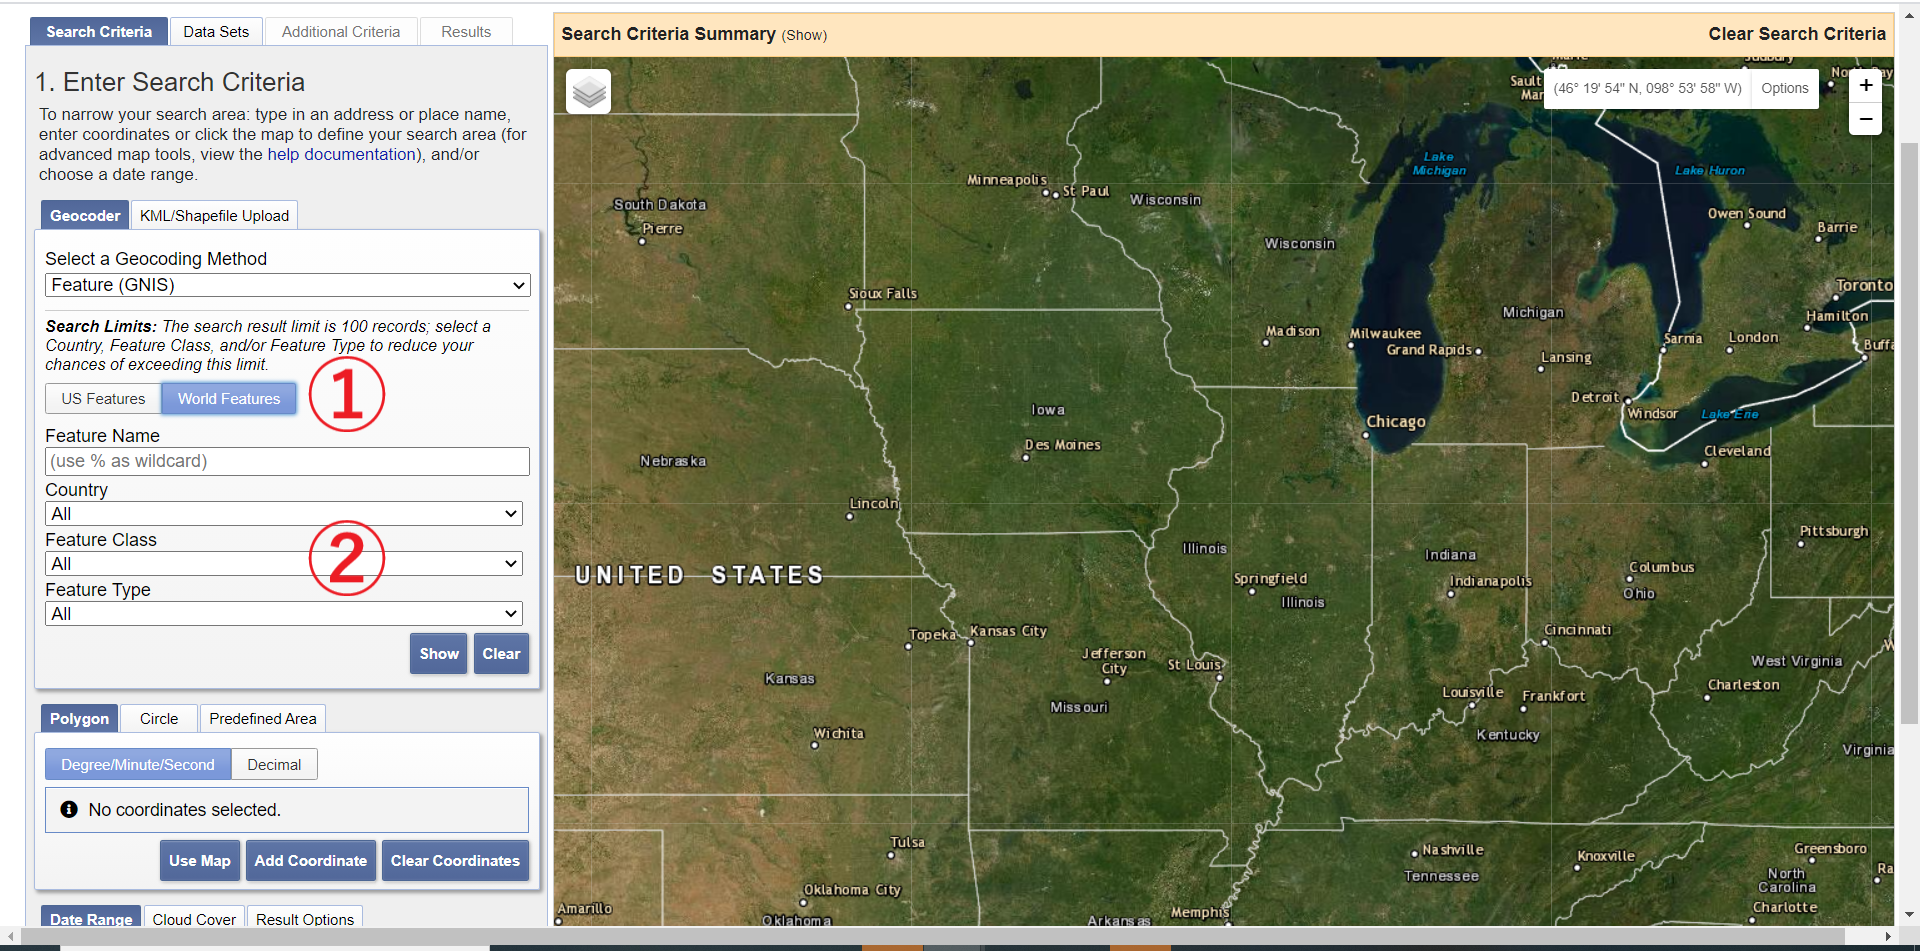
\includegraphics{images/area1.png}
③【Show】を押下すると、下図のような表が表示されるので、自分がデータを取得したい地点を選択する.
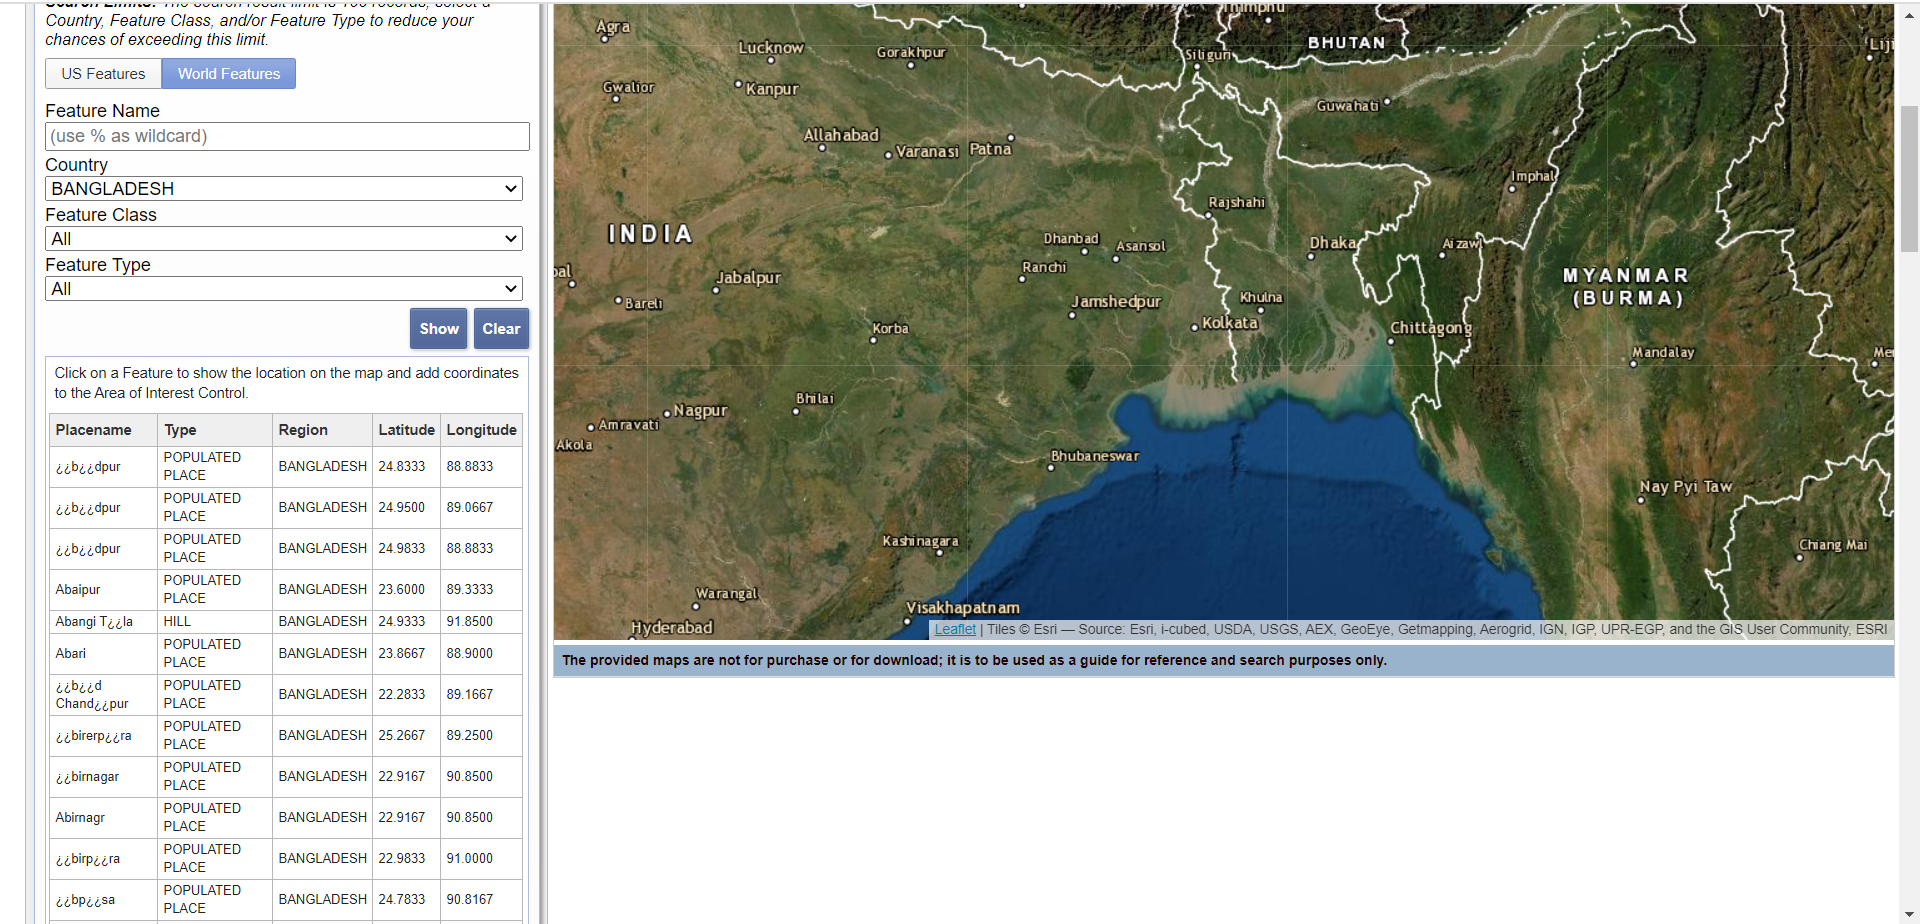
\includegraphics{images/table1.png}

④地点を選択すると、下図のように右地図エリアにもポイントが表れる.
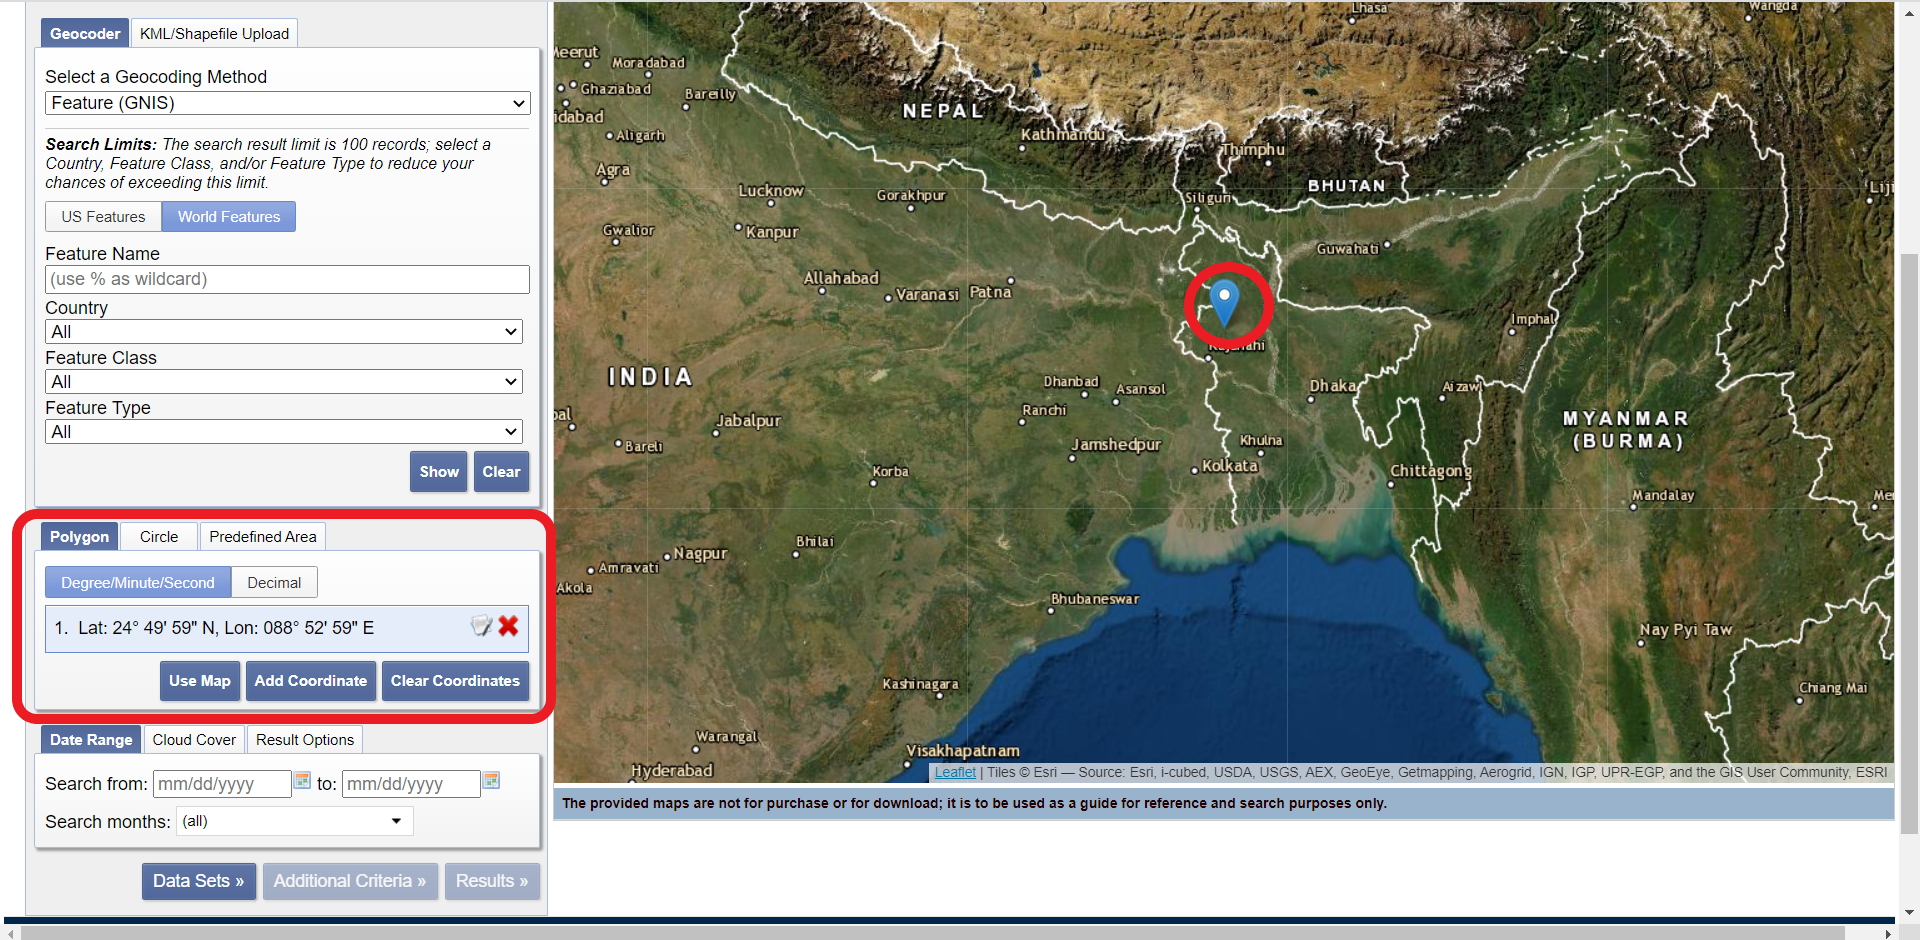
\includegraphics{images/showarea.png}

\begin{itemize}
\tightlist
\item
  広範囲の衛星画像データを取得したい場合
\end{itemize}

\textbf{【Polygon】}  

①【Polygon】を選択.

②右地図エリアで、データを取得したい地域を囲うように各地点をクリックしていく.\\
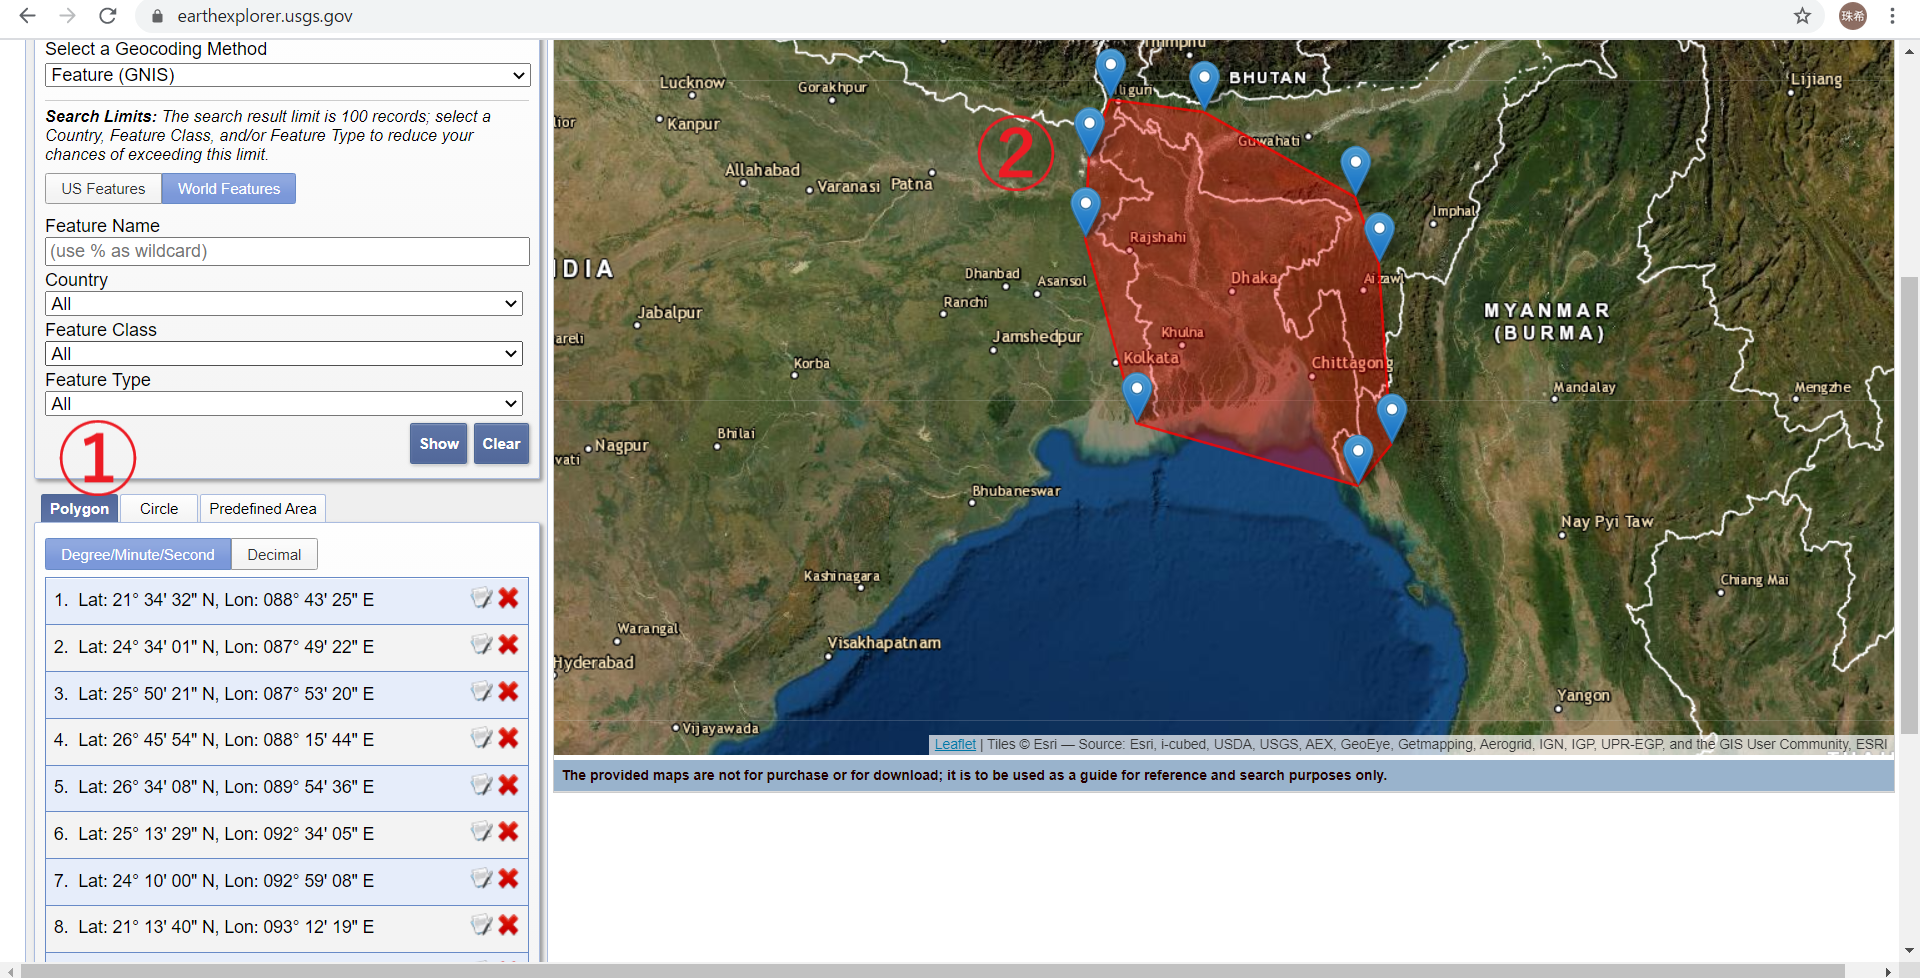
\includegraphics{images/polygon.png}

\textbf{【Circle】}

①【Circle】を選択 .

②右地図エリアから適当に1地点をクリックする.データを取得したい地域に合わせて、もう1地点をクリックする.\\
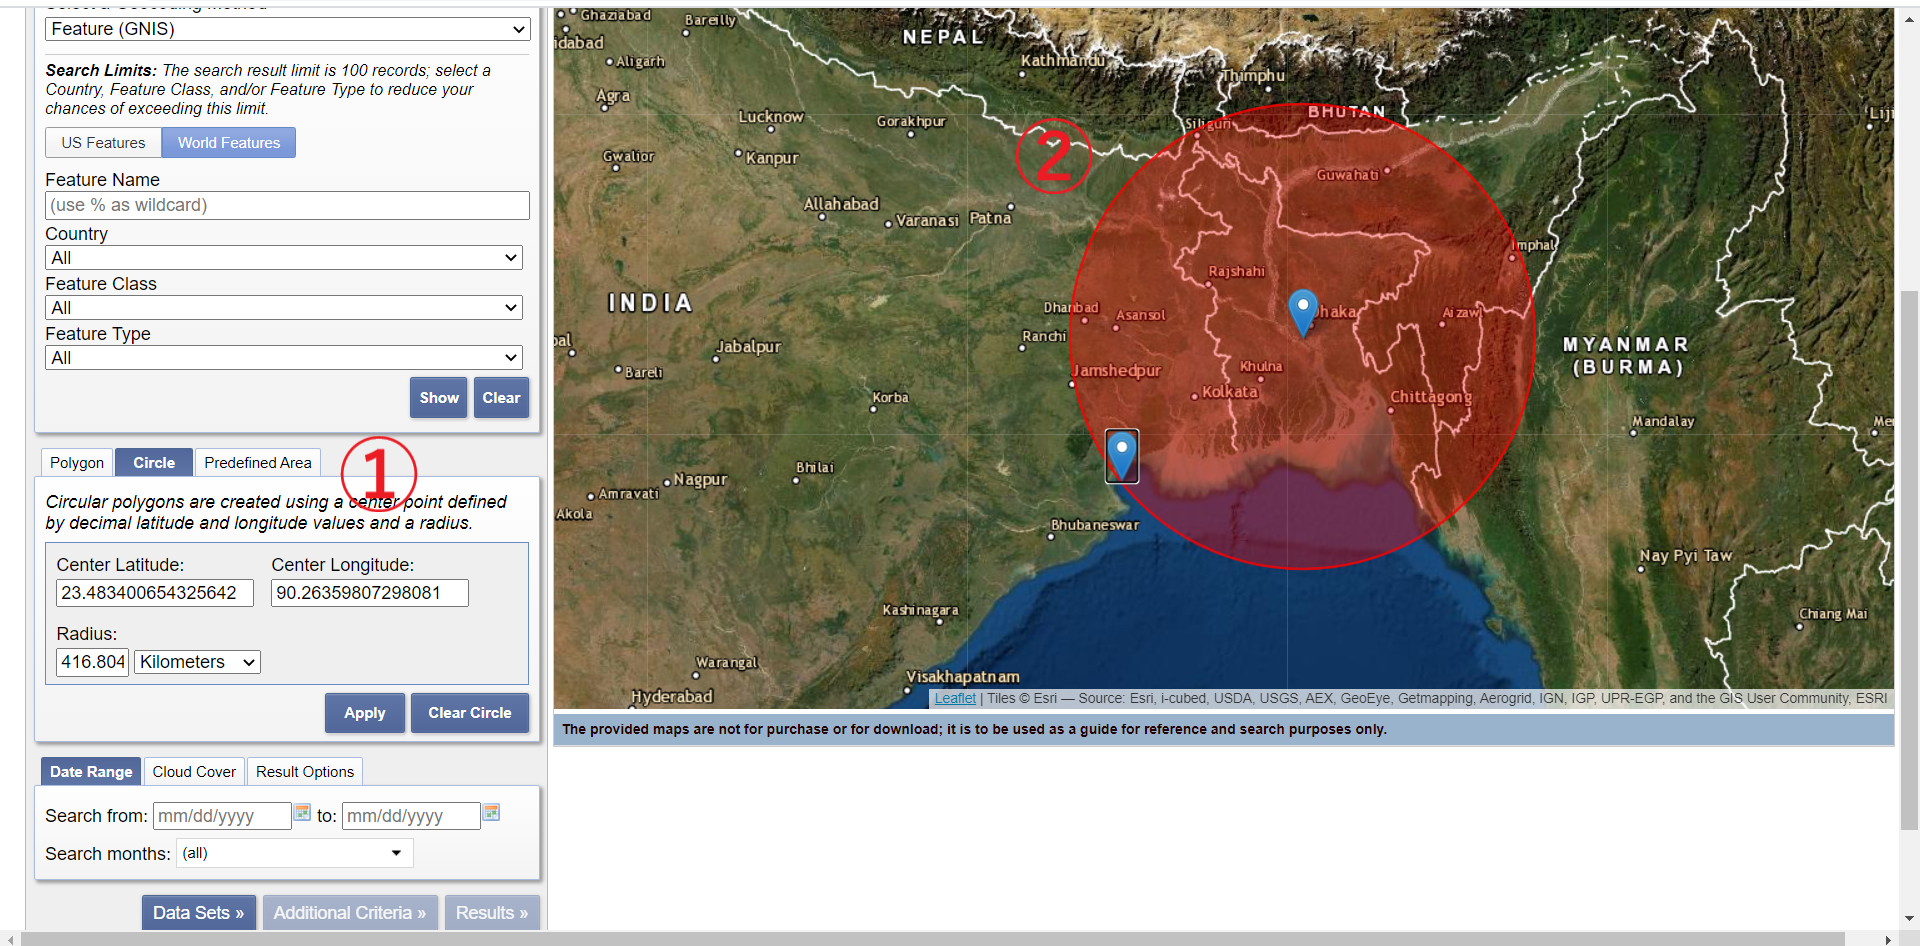
\includegraphics{images/circle1.png}
③【Apply】を押下.

\hypertarget{ux30c7ux30fcux30bfux3092ux53d6ux5f97ux3057ux305fux3044ux65e5ux6642ux3092ux8a2dux5b9aux3059ux308b}{%
\section{データを取得したい日時を設定する}\label{ux30c7ux30fcux30bfux3092ux53d6ux5f97ux3057ux305fux3044ux65e5ux6642ux3092ux8a2dux5b9aux3059ux308b}}

【Date Range】から選択
(カレンダーから選択が可能)
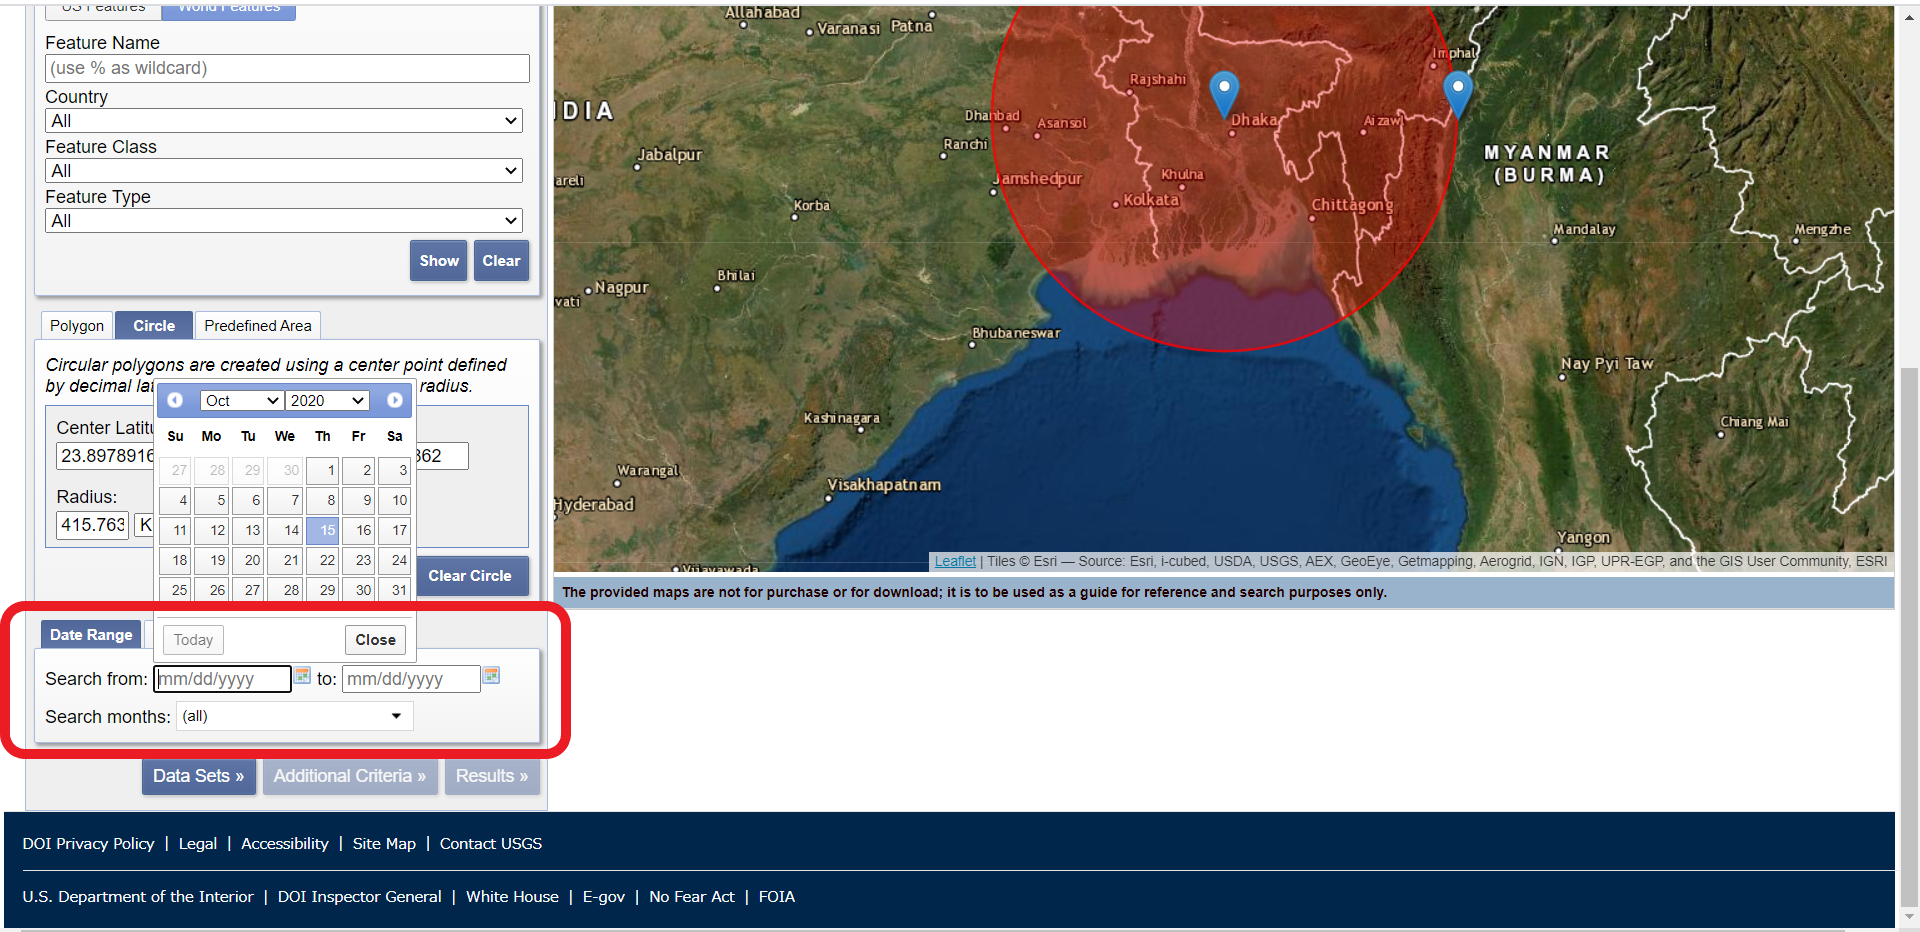
\includegraphics{images/date.png}

\hypertarget{ux96f2ux306eux91cfux3092ux8abfux6574ux3059ux308b}{%
\section{雲の量を調整する}\label{ux96f2ux306eux91cfux3092ux8abfux6574ux3059ux308b}}

【Cloud Cover】でバーを動かすことにより、設定が可能
*ただし衛星データによっては雲量調整を行っていないものがあり、その場合は適用されない.\\
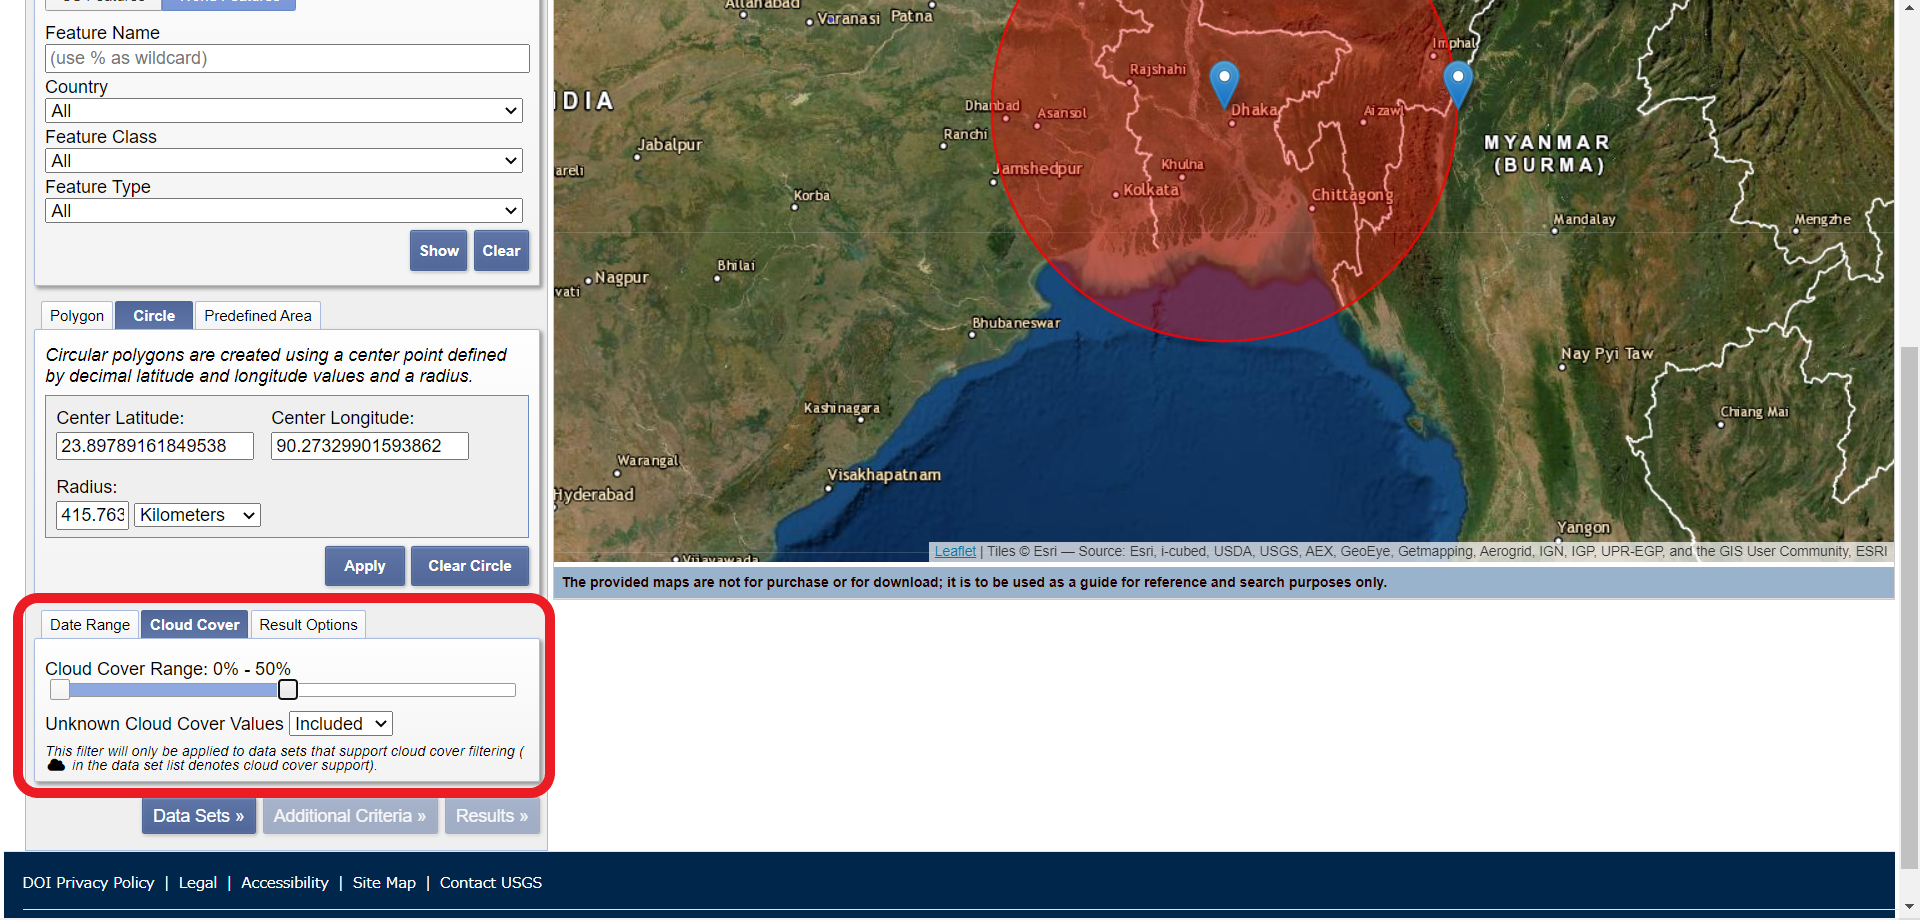
\includegraphics{images/cloud.png}

\hypertarget{data-setsux3092ux62bcux4e0b}{%
\section{【Data Sets】を押下}\label{data-setsux3092ux62bcux4e0b}}

\hypertarget{ux5fc5ux8981ux306aux30c7ux30fcux30bfux30bbux30c3ux30c8ux3092ux9078ux629eux3059ux308b}{%
\section{必要なデータセットを選択する}\label{ux5fc5ux8981ux306aux30c7ux30fcux30bfux30bbux30c3ux30c8ux3092ux9078ux629eux3059ux308b}}

データセットの中から必要なデータセットを選択する

今回は、冒頭のとおり、MODIS Vegetation Index Productsを選択します.

*データセット名の左のインフォメーションマークを押下すると説明が出る

*データセット名の左の地図マークを押下すると、そのデータのカバー範囲が右地図上に表示される\\
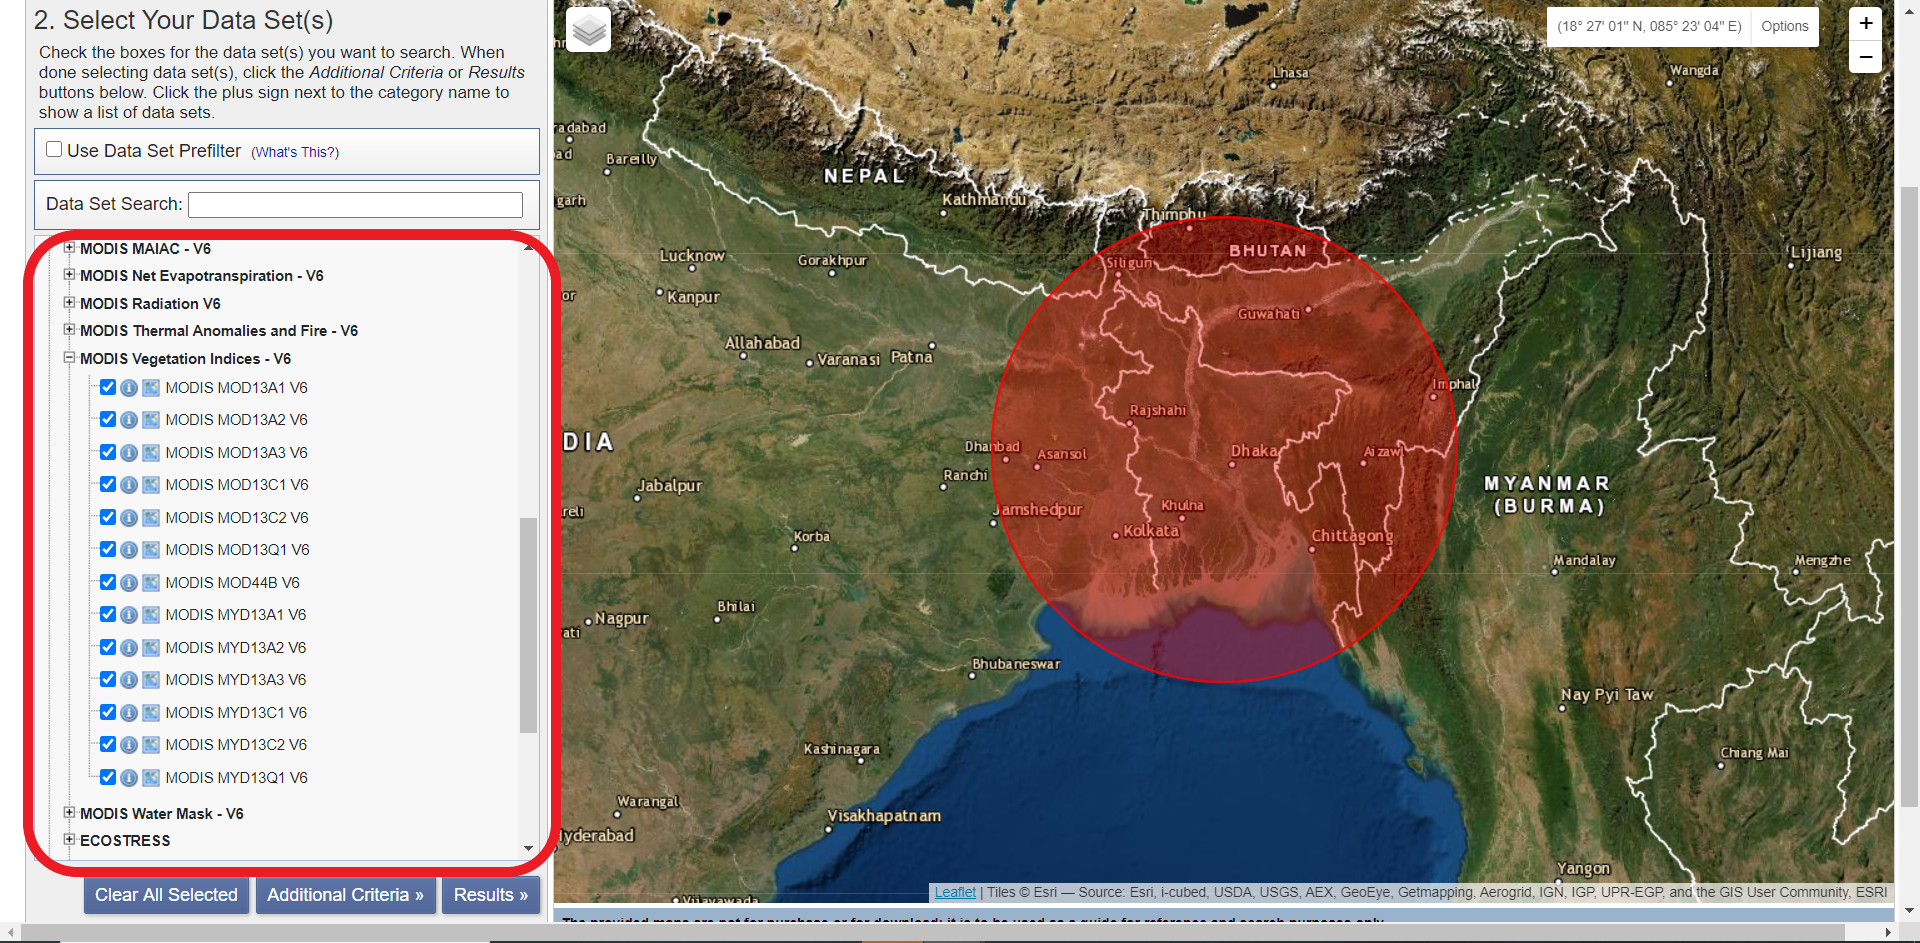
\includegraphics{images/datasets.png}

\hypertarget{resultsux3092ux62bcux4e0b}{%
\section{【Results】を押下}\label{resultsux3092ux62bcux4e0b}}

\hypertarget{ux30c7ux30fcux30bfux306eux30c0ux30a6ux30f3ux30edux30fcux30c9}{%
\section{データのダウンロード}\label{ux30c7ux30fcux30bfux306eux30c0ux30a6ux30f3ux30edux30fcux30c9}}

\begin{itemize}
\tightlist
\item
  【Show Brouwse Overlay】を押下すると、各データを右地図上に表示することができる
  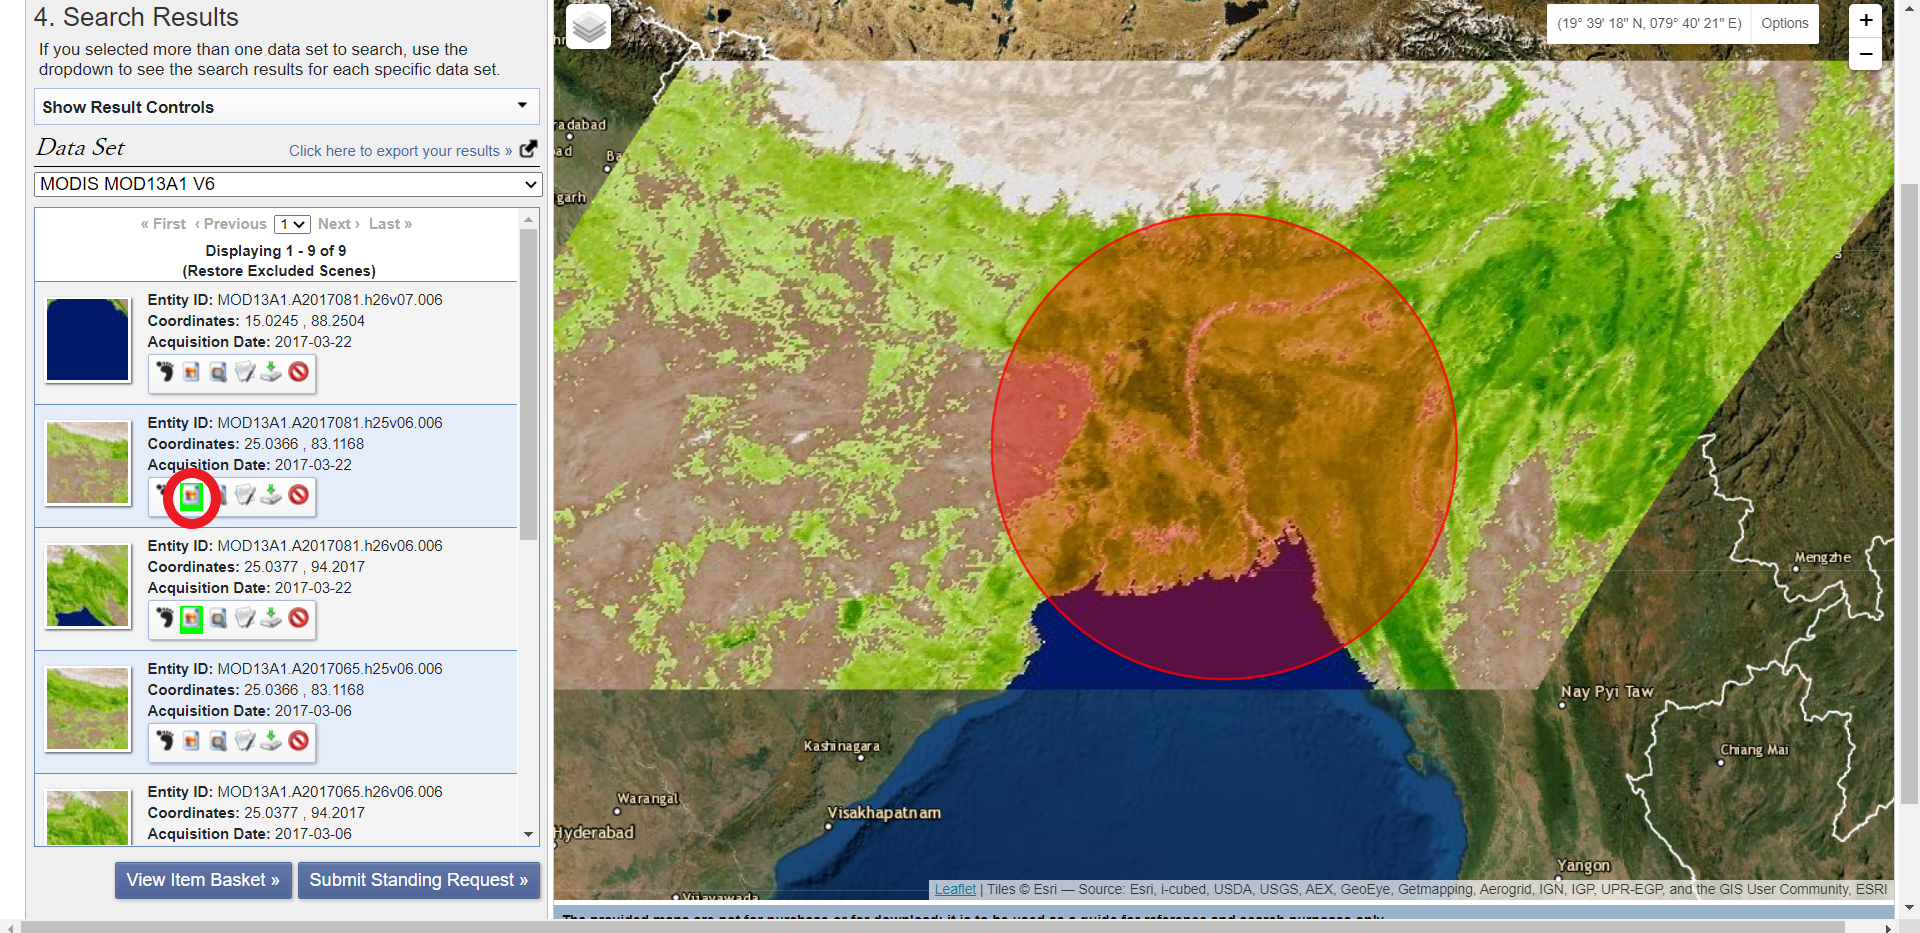
\includegraphics{images/overray.png}
\end{itemize}

*複数のデータにわたる場合には、Acquisition Dateを確認する(データの詳細は【Show Mwtadata and Browse】から確認可能)

\begin{itemize}
\item
  【Click here to export your results】の【Export data】を押下.\\
  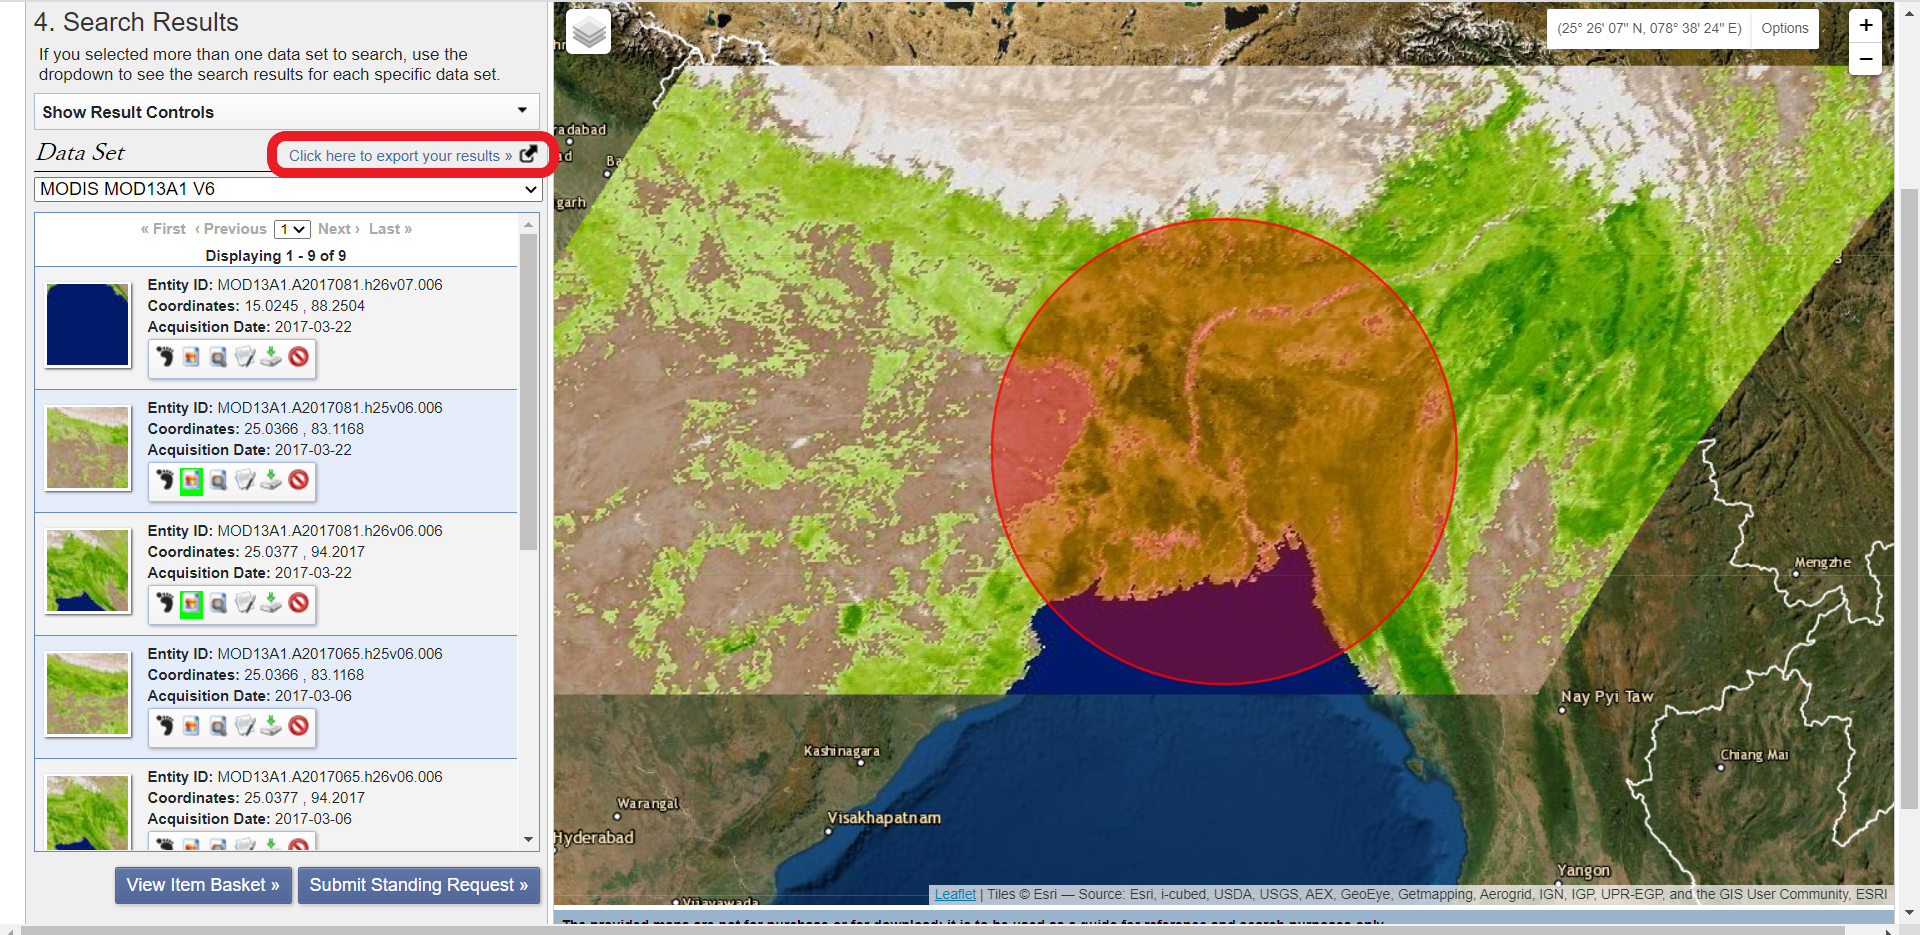
\includegraphics{images/download.png}
\item
  【Export name】,【Export file】を設定する.
\item
  【Download】を押下. HDFファイルでのダウンロードとなる。
  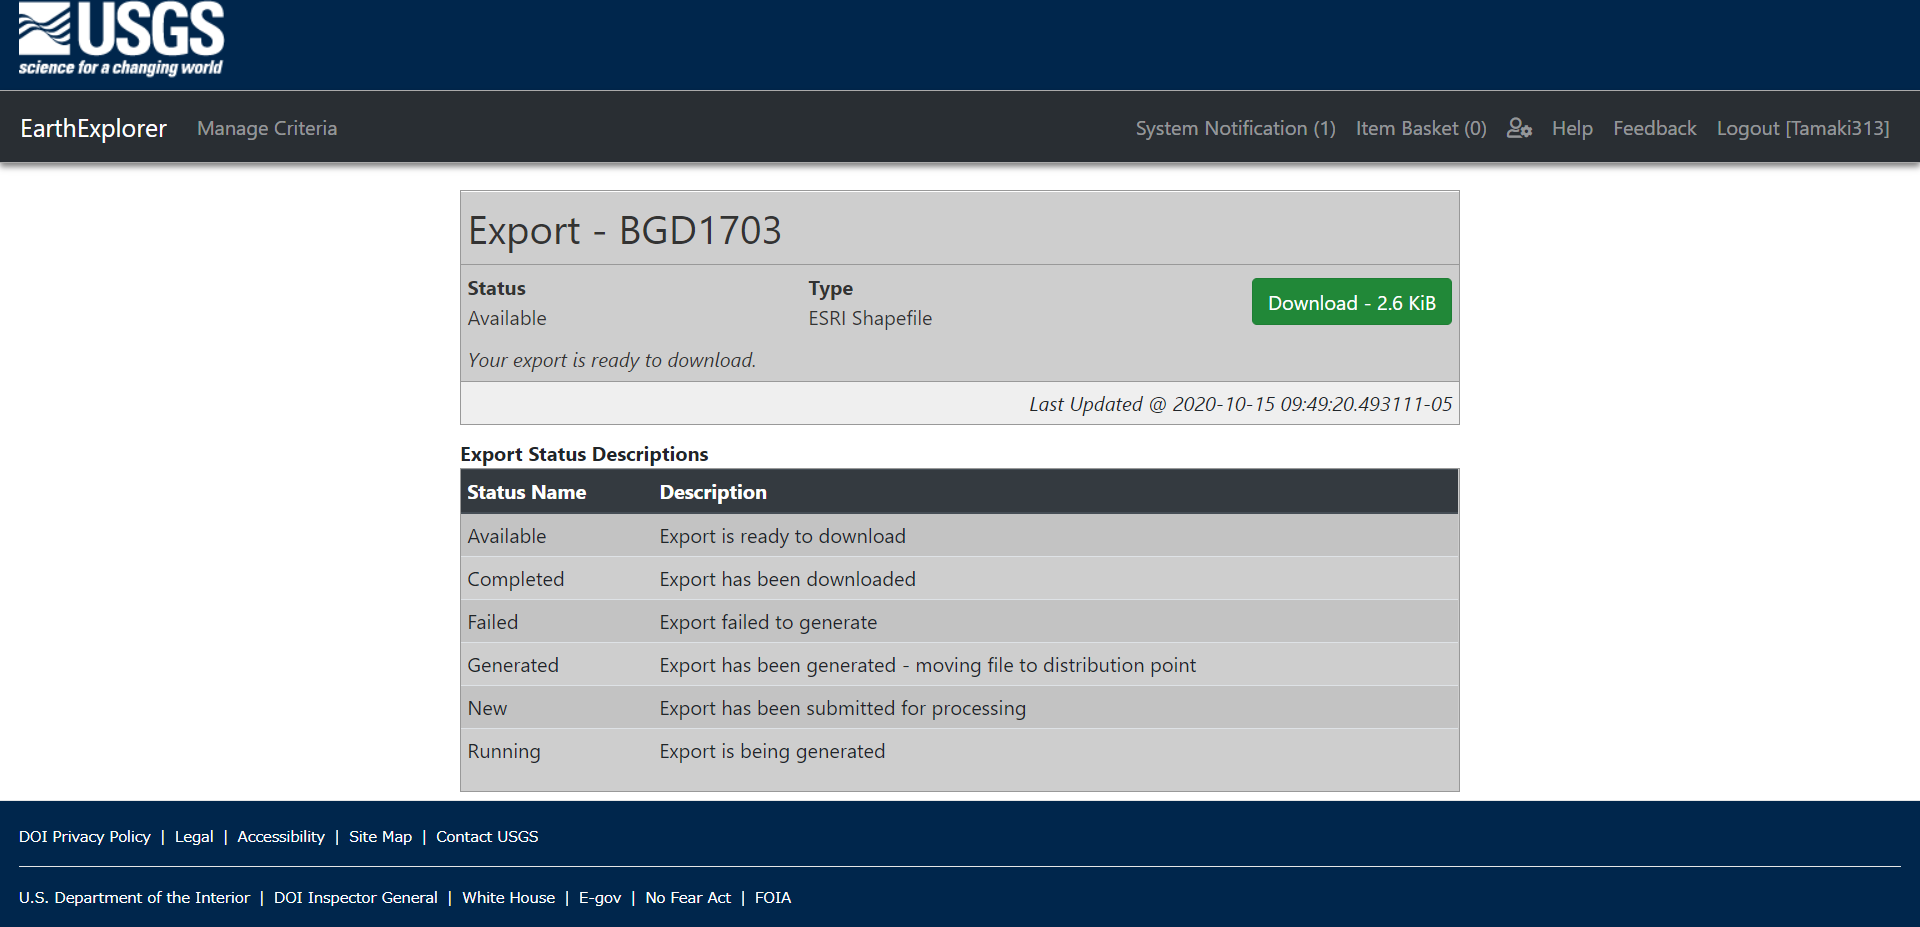
\includegraphics{images/last.png}
\end{itemize}

\hypertarget{ux885bux661fux30c7ux30fcux30bfux306eux53d6ux5f97ux65b9ux6cd5laads-daacux7de8}{%
\chapter{衛星データの取得方法(LAADS DAAC編)}\label{ux885bux661fux30c7ux30fcux30bfux306eux53d6ux5f97ux65b9ux6cd5laads-daacux7de8}}

今回は、LAADS DAACを利用して、BangladeshのMODIS Vegetation Index Productsをダウンロードする方法をご紹介します。

MODIS: NASAによって開発された可視・赤外域の放射計で、地球観測衛星のTerra、Aquaに搭載されている。\\
Vegetation Index Products: 植物による光の反射の特徴を生かし、植生の状況を把握することを目的とした指標

\hypertarget{laads-daacux306bux767bux9332ux30edux30b0ux30a4ux30f3ux3059ux308b}{%
\section{LAADS DAACに登録/ログインする}\label{laads-daacux306bux767bux9332ux30edux30b0ux30a4ux30f3ux3059ux308b}}

LAADS DAACから取得できるデータ  

\begin{itemize}
\item
  MODIS(最新データ日時:2020年9月29日)  
\item
  AVHRR
\item
  ESA copernics-sentinel-3
\item
  MERIS
\item
  VIIRS
\end{itemize}

\hypertarget{find-dataux3092ux62bcux3059}{%
\section{【Find Data】を押す}\label{find-dataux3092ux62bcux3059}}

\begin{figure}
\centering
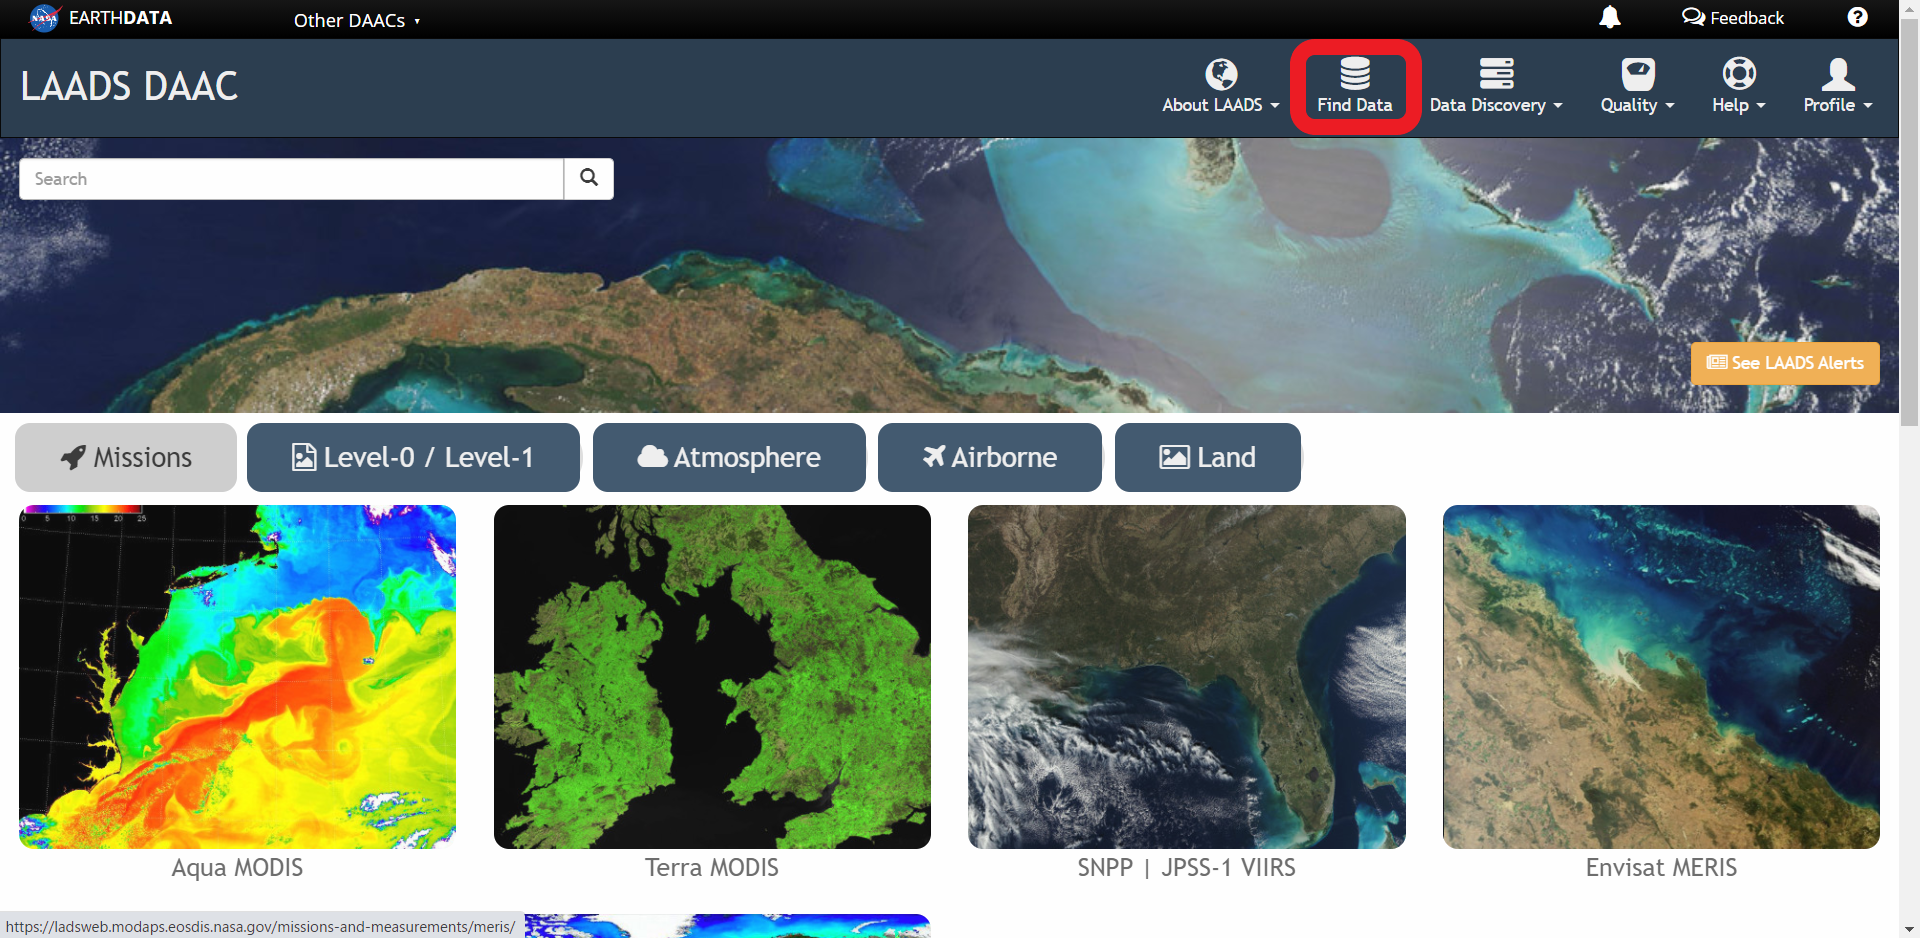
\includegraphics{images/LD-1.png}
\caption{find data}
\end{figure}

\hypertarget{productsux5fc5ux8981ux306aux30c7ux30fcux30bfux3092ux9078ux629eux3059ux308b}{%
\section{①PRODUCTS:必要なデータを選択する}\label{productsux5fc5ux8981ux306aux30c7ux30fcux30bfux3092ux9078ux629eux3059ux308b}}

ここではMOD13A1,MYD13A1を選択した。
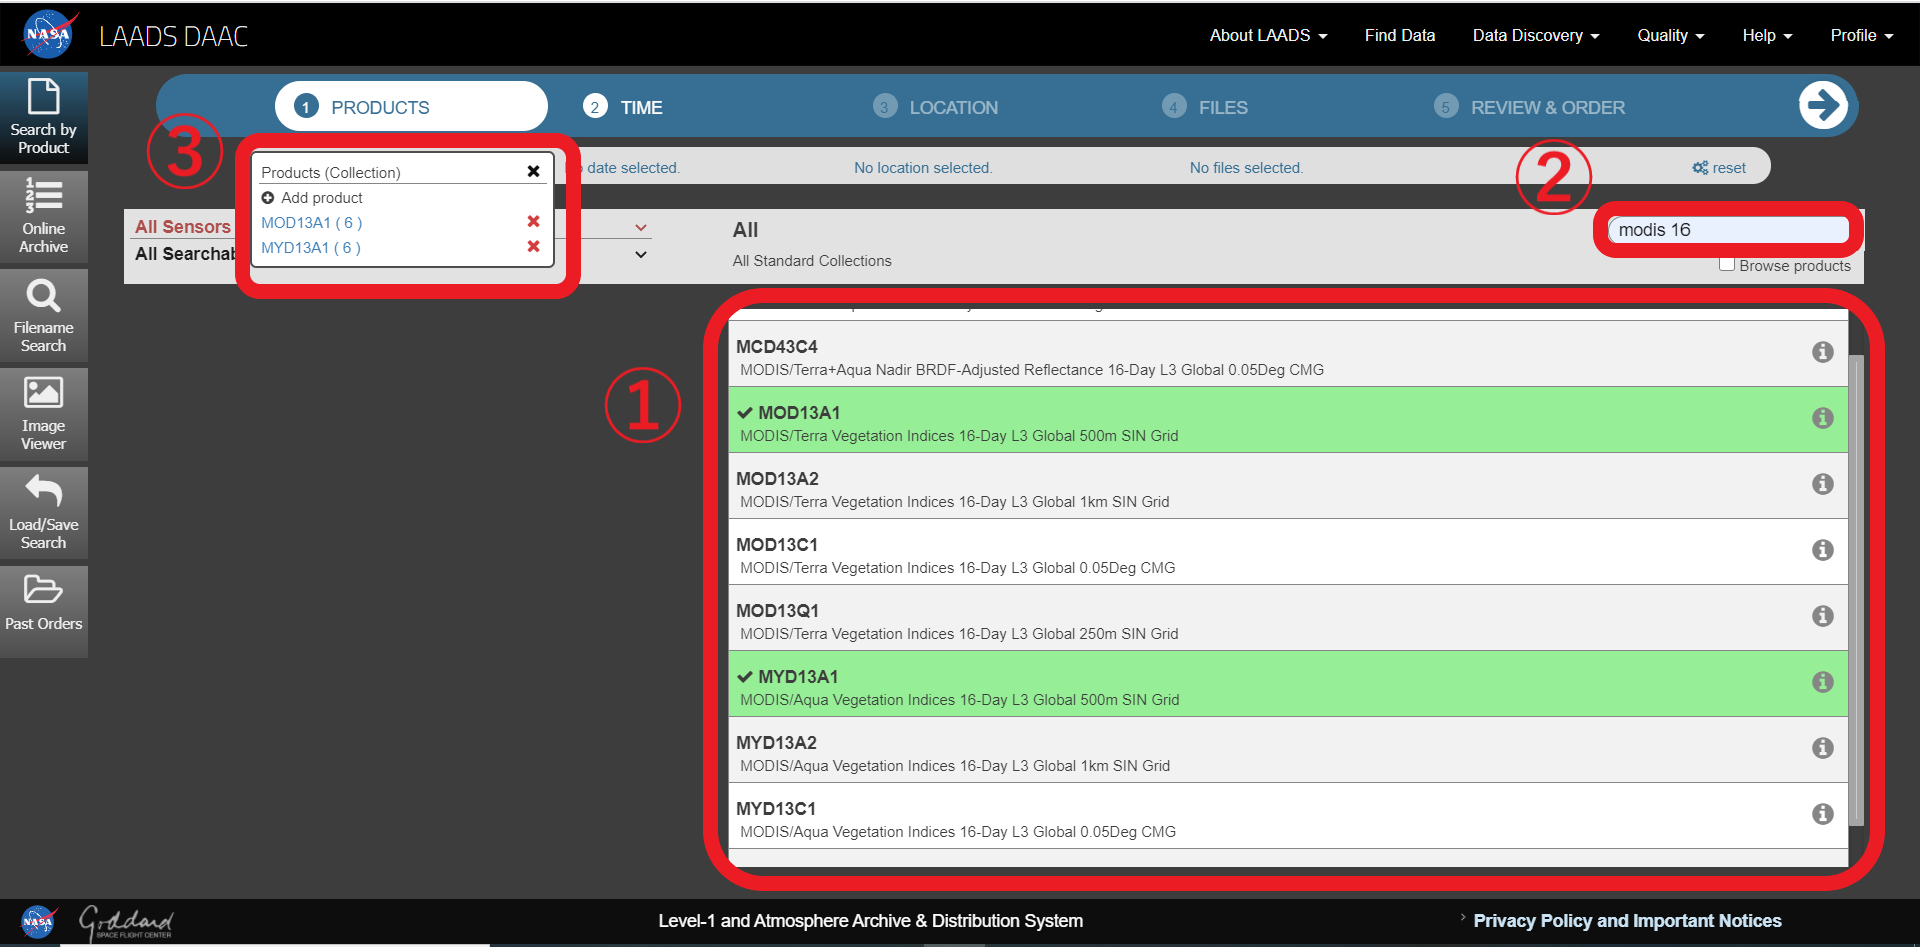
\includegraphics{images/LD-2.png}

\hypertarget{timeux53d6ux5f97ux3057ux305fux3044ux30c7ux30fcux30bfux306eux65e5ux6642ux3092ux8a2dux5b9aux3059ux308b}{%
\section{②TIME:取得したいデータの日時を設定する}\label{timeux53d6ux5f97ux3057ux305fux3044ux30c7ux30fcux30bfux306eux65e5ux6642ux3092ux8a2dux5b9aux3059ux308b}}

ここでは2017年3月1日から2017年3月31日を設定。

必ず【Add date】を押す。
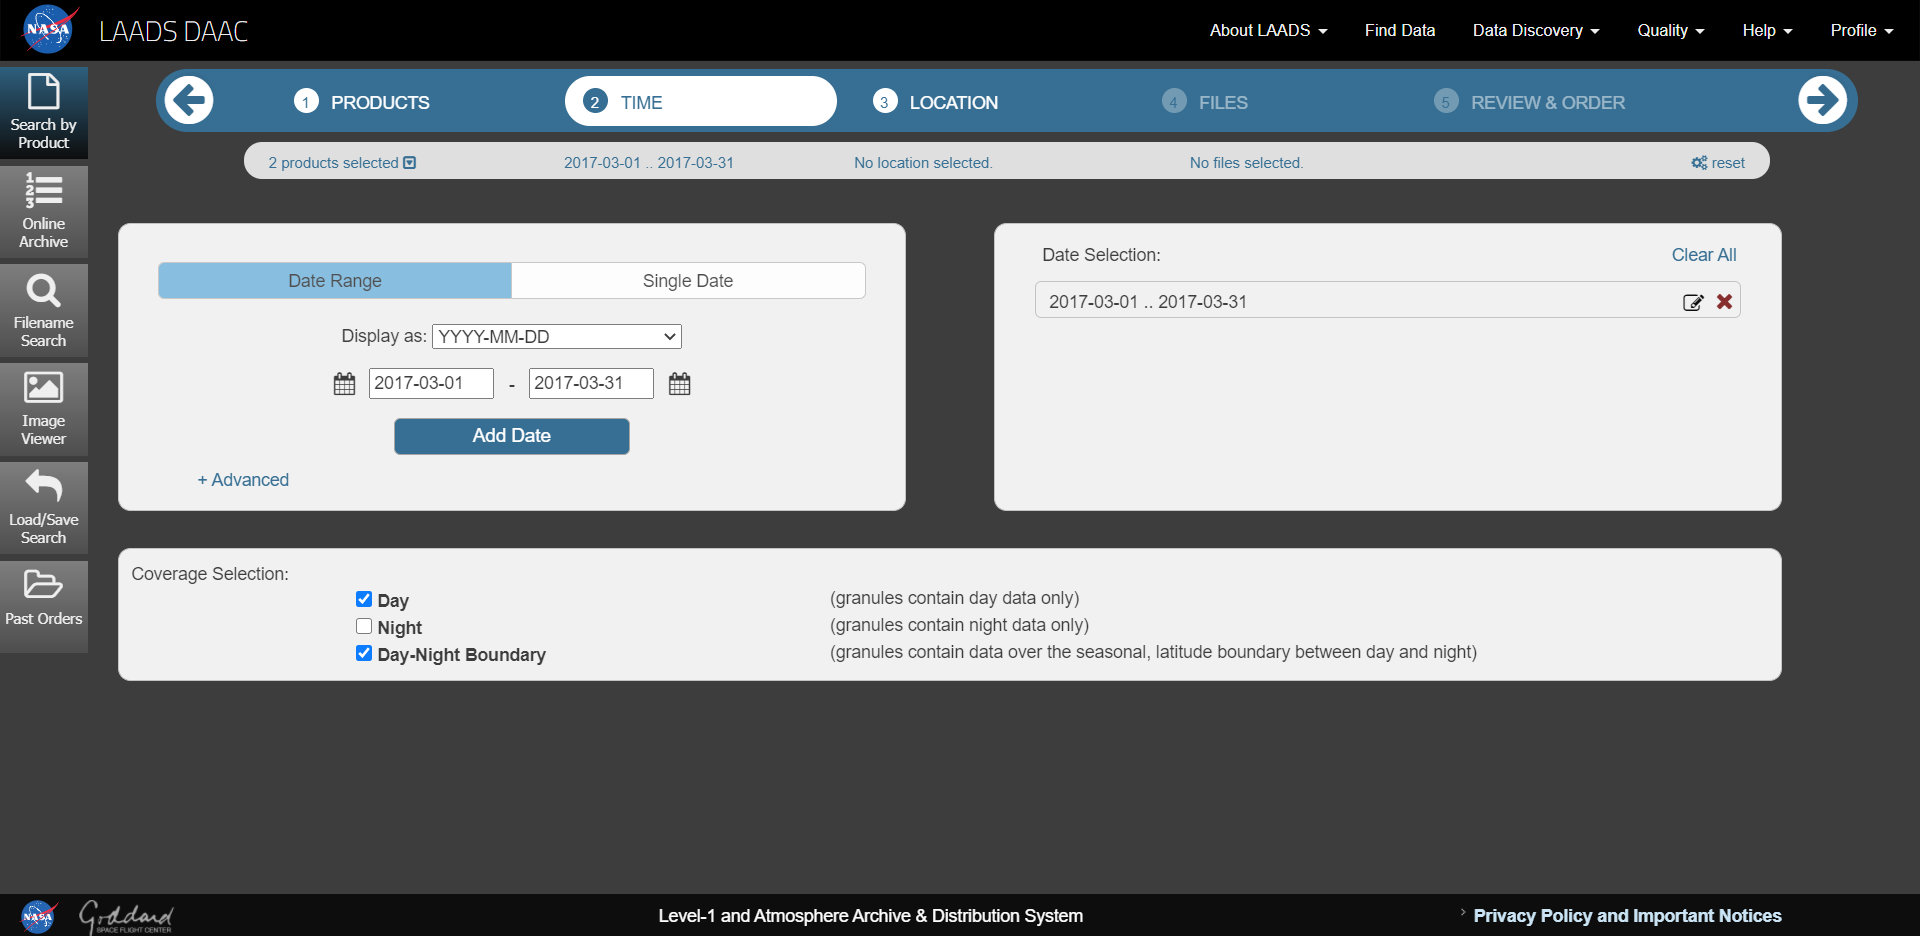
\includegraphics{images/LD-3.png}

\hypertarget{locationux53d6ux5f97ux3057ux305fux3044ux30c7ux30fcux30bfux306eux5730ux57dfux3092ux8a2dux5b9aux3059ux308b}{%
\section{③LOCATION:取得したいデータの地域を設定する}\label{locationux53d6ux5f97ux3057ux305fux3044ux30c7ux30fcux30bfux306eux5730ux57dfux3092ux8a2dux5b9aux3059ux308b}}

ここではバングラデシュを選択する。

【Countries】を押すと、国境が表示されるので、データを取得したい国を選択する。

そのほかにも、全世界や自分で地域を設定することも可能。
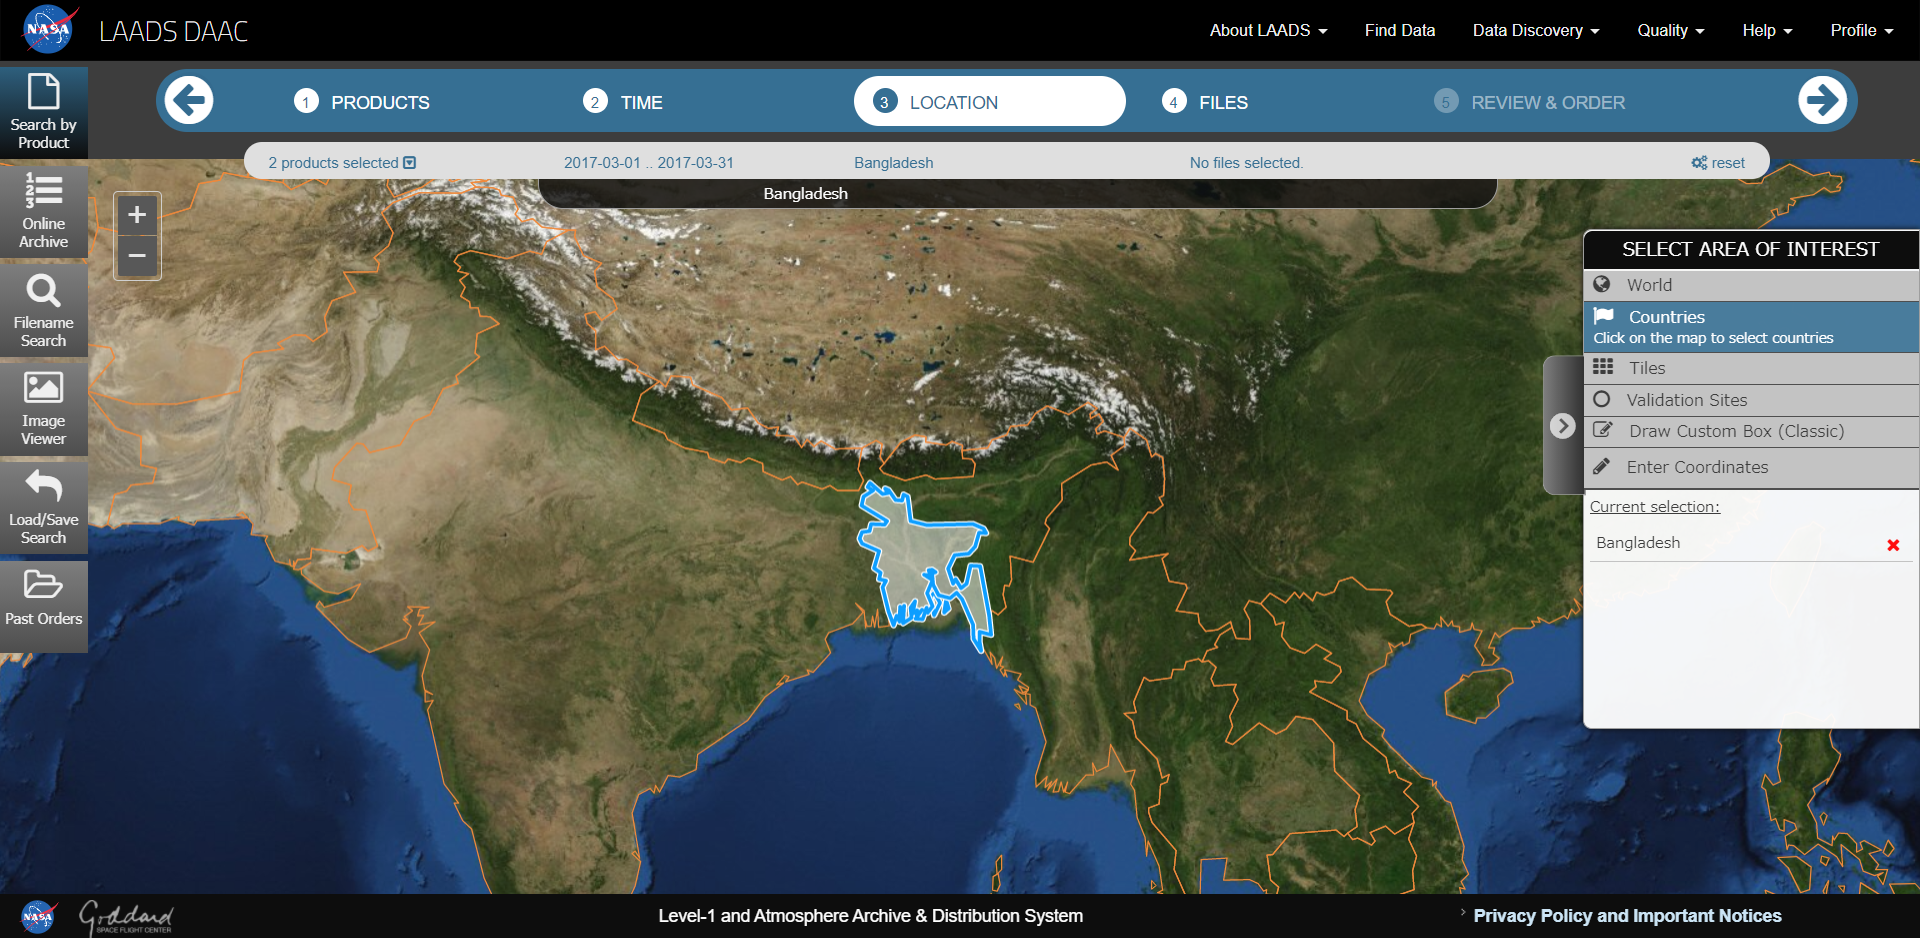
\includegraphics{images/LD-4.png}

\hypertarget{filesux8868ux793aux3055ux308cux305fux30d5ux30a1ux30a4ux30ebux304bux3089ux5fc5ux8981ux306aux3082ux306eux3092ux9078ux629eux3059ux308b}{%
\section{④FILES:表示されたファイルから必要なものを選択する}\label{filesux8868ux793aux3055ux308cux305fux30d5ux30a1ux30a4ux30ebux304bux3089ux5fc5ux8981ux306aux3082ux306eux3092ux9078ux629eux3059ux308b}}

ここでファイルの左にある【Download】を押すとHDFファイルのダウンロードが可能。
GeoTIFF形式に変更したい場合は、以下の操作を行う。

\begin{figure}
\centering
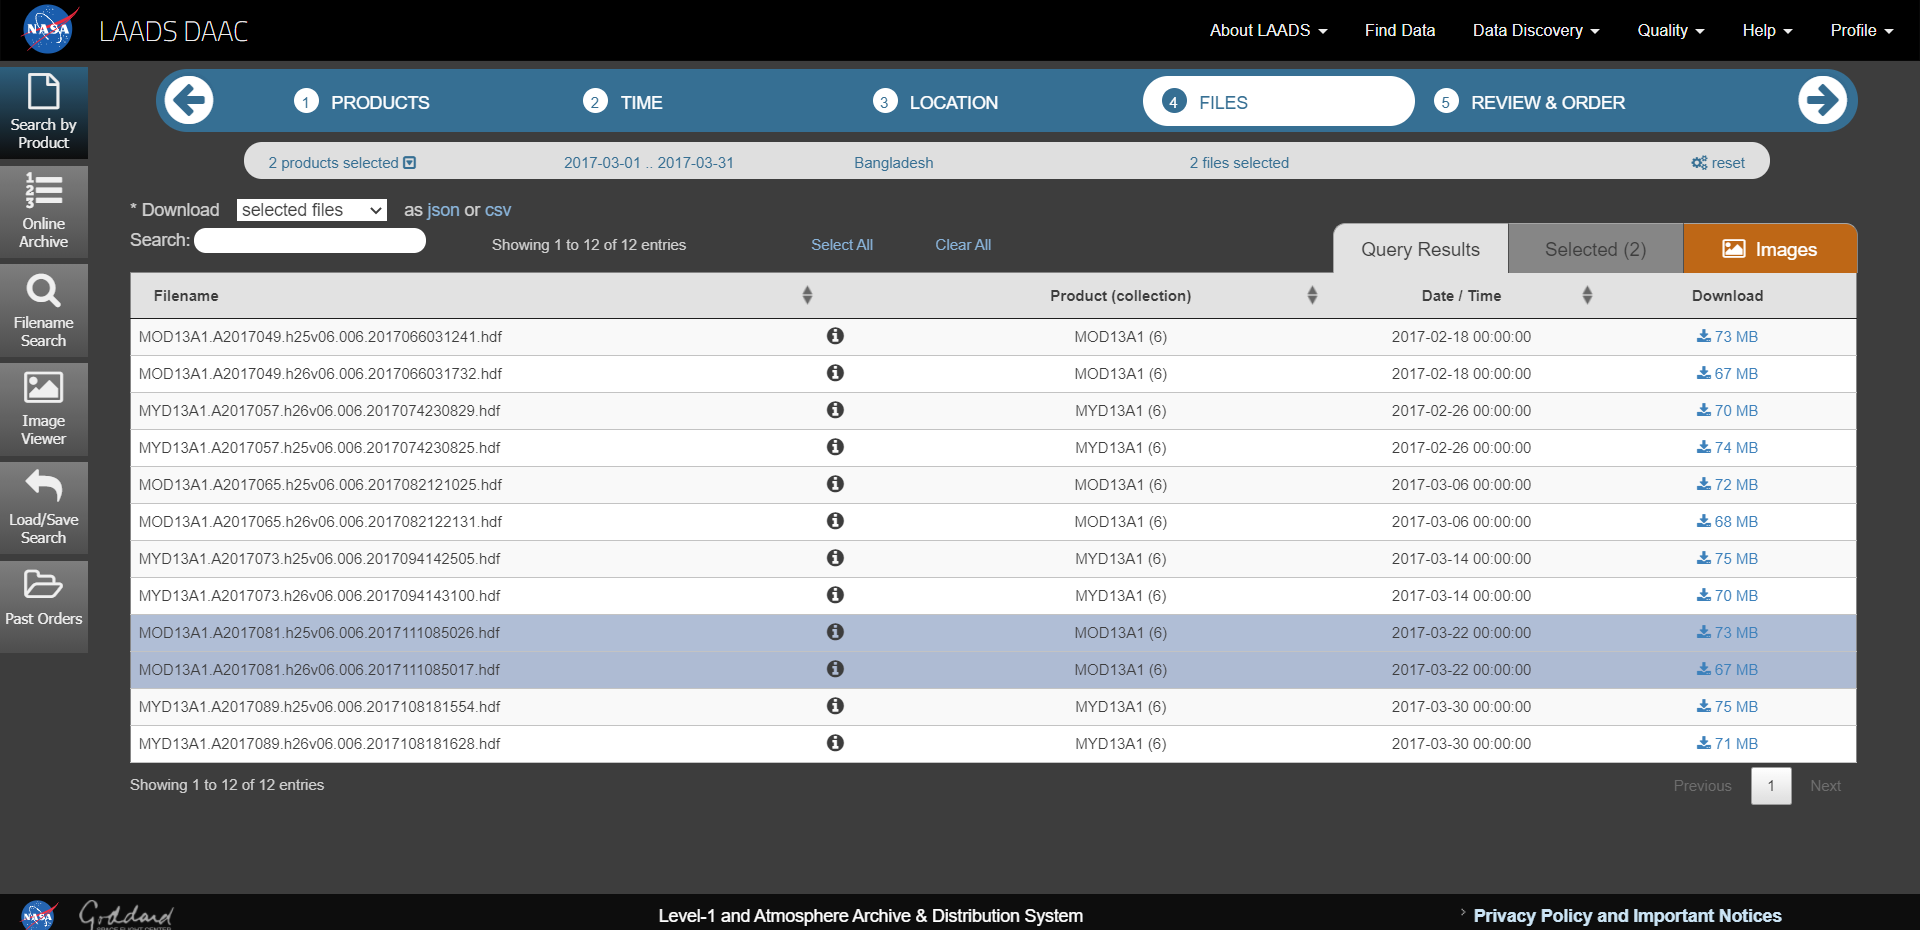
\includegraphics{images/LD-5.png}
\caption{files}
\end{figure}

\hypertarget{revieworderux30d5ux30a1ux30a4ux30ebux306eux5f62ux5f0fux306aux3069ux3092ux6307ux5b9aux3057ux30c0ux30a6ux30f3ux30edux30fcux30c9ux3059ux308b}{%
\section{⑤REVIEW\&ORDER:ファイルの形式などを指定し、ダウンロードする}\label{revieworderux30d5ux30a1ux30a4ux30ebux306eux5f62ux5f0fux306aux3069ux3092ux6307ux5b9aux3057ux30c0ux30a6ux30f3ux30edux30fcux30c9ux3059ux308b}}

【Apply Post-Processing】を押す。

今回はNDVIのデータを取得できれば良いので、【SDs】を押し、【500m 16days NDVI】を選択する。
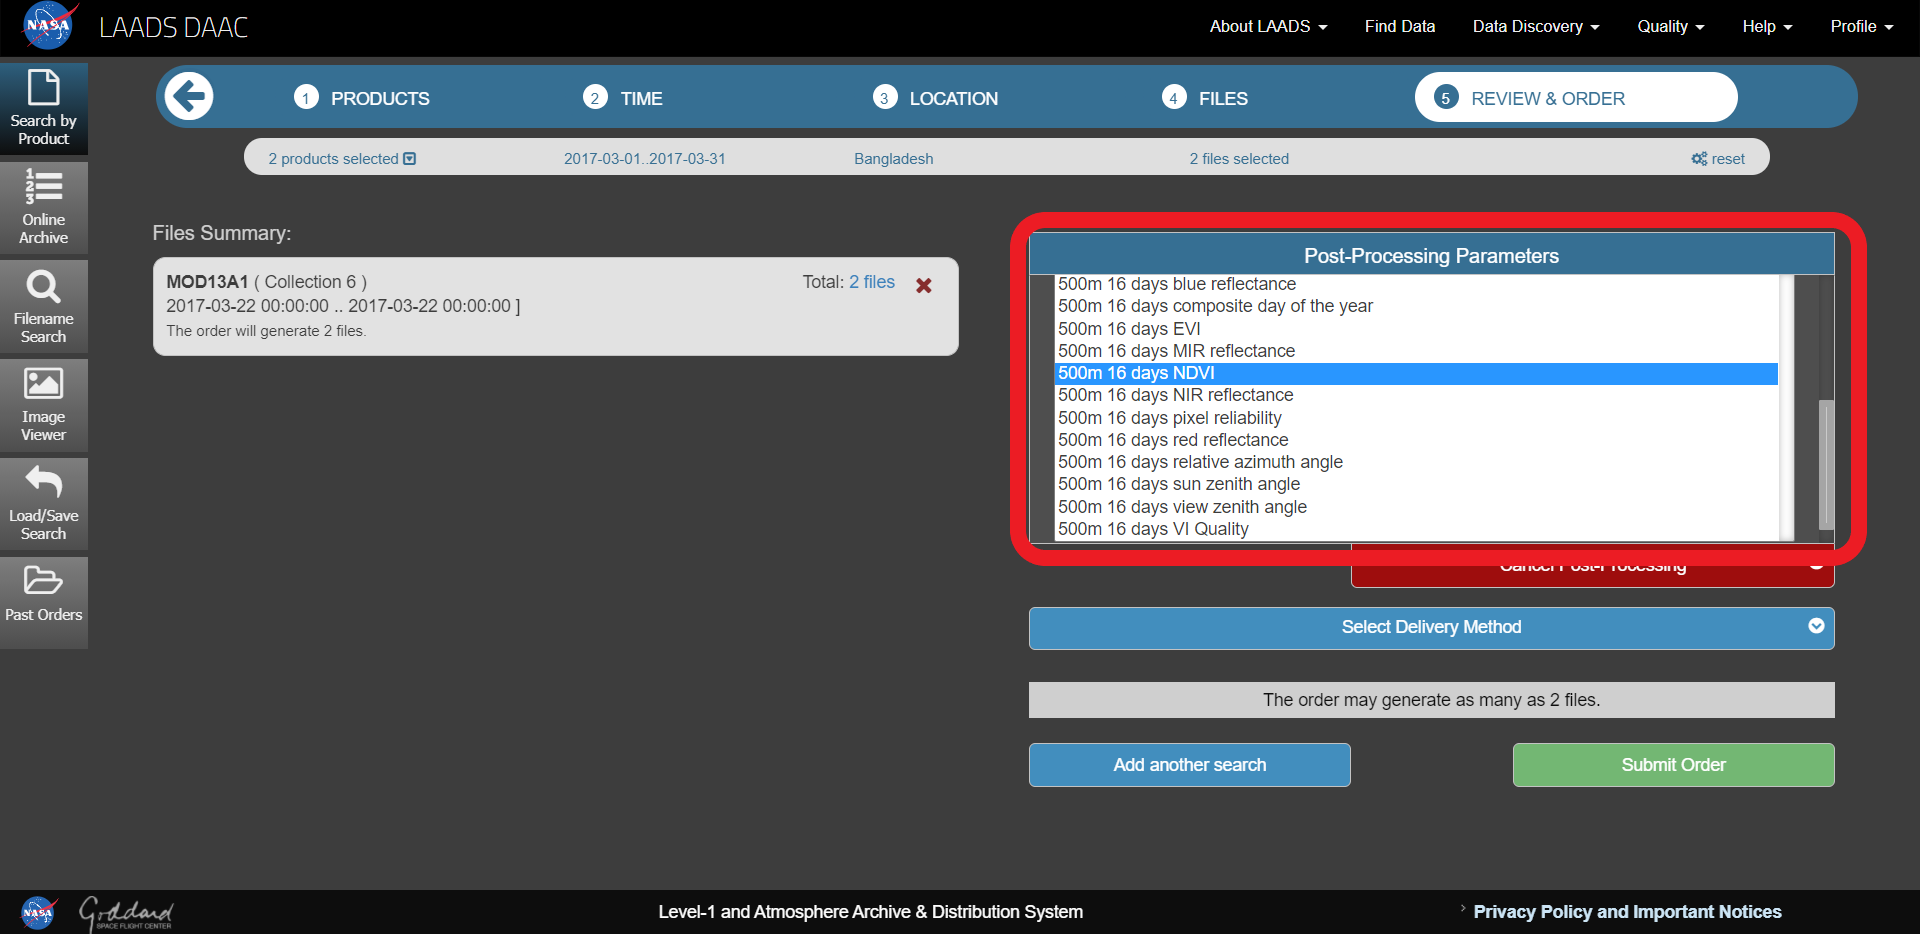
\includegraphics{images/LD-6.png}

【Reformat】を押し、【Convert products to geoTIFF format】にチェックを入れる。
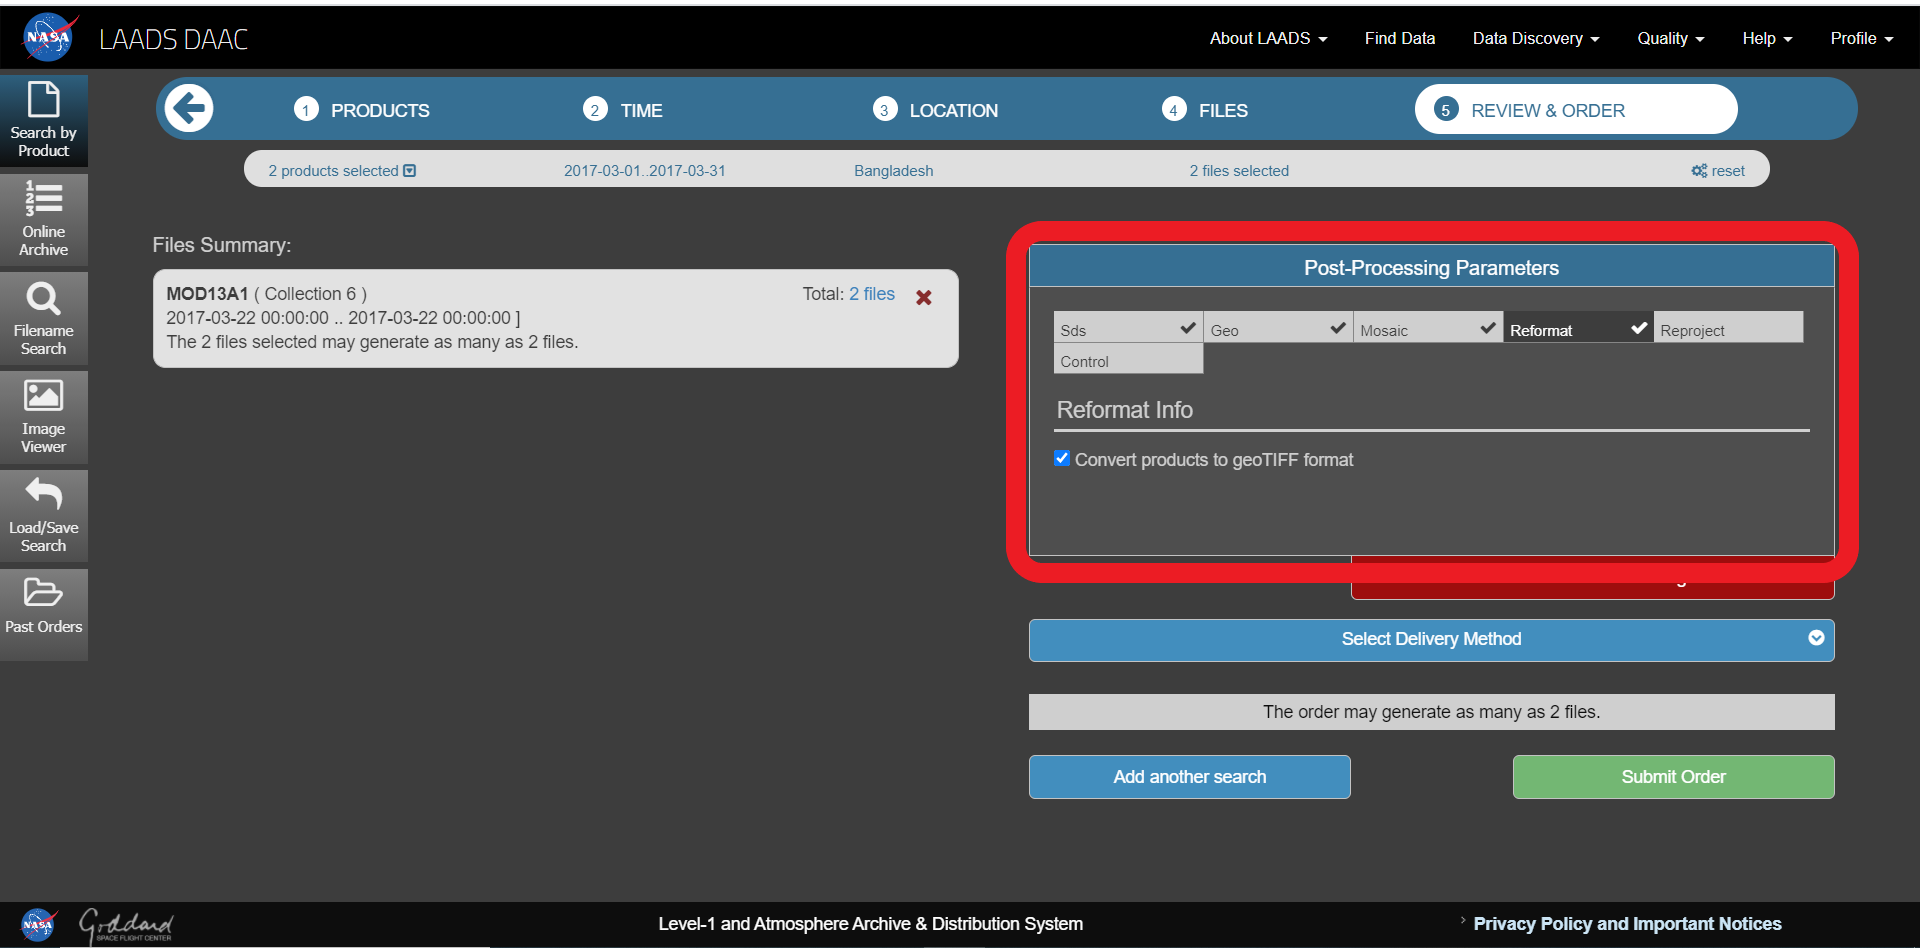
\includegraphics{images/LD-7.png}

\hypertarget{submit-orderux3092ux62bcux3059}{%
\section{【Submit Order】を押す}\label{submit-orderux3092ux62bcux3059}}

5分程度で登録しているメールアドレスに``LAADS Web Order Notification''というタイトルのメールが届くので、文中のURLからダウンロードを行う。

\hypertarget{ux6d78ux6c34ux30deux30c3ux30d7ux306eux4f5cux6210}{%
\chapter{浸水マップの作成}\label{ux6d78ux6c34ux30deux30c3ux30d7ux306eux4f5cux6210}}

洪水時の浸水状況を把握するためのマップを、Google earth engineを使って作成してみましょう。  

\hypertarget{google-earth-engineux306bux3064ux3044ux3066}{%
\section{Google earth engineについて}\label{google-earth-engineux306bux3064ux3044ux3066}}

Google earth engineとは、衛星画像をGoogleクラウド上で解析・利用できるサービス。  
*研究・教育・非営利目的ならば無料で利用可能。  

Google earth engineは、以下の点で画期的と言われています。  

\begin{itemize}
\item
  前処理済みデータ(ARD)を入手できる  
\item
  容量の大きなデータをダウンロードすることなく、解析することが可能  
\end{itemize}

それでは早速、Google earth engineに登録してみましょう。  

(Googleアカウントを所持していない場合)Googleアカウントを登録する  

Google earth engineの【Sign up】タブからログイン 

\hypertarget{gee-code-editorux306eux4f7fux7528}{%
\section{GEE CODE EDITORの使用  }\label{gee-code-editorux306eux4f7fux7528}}

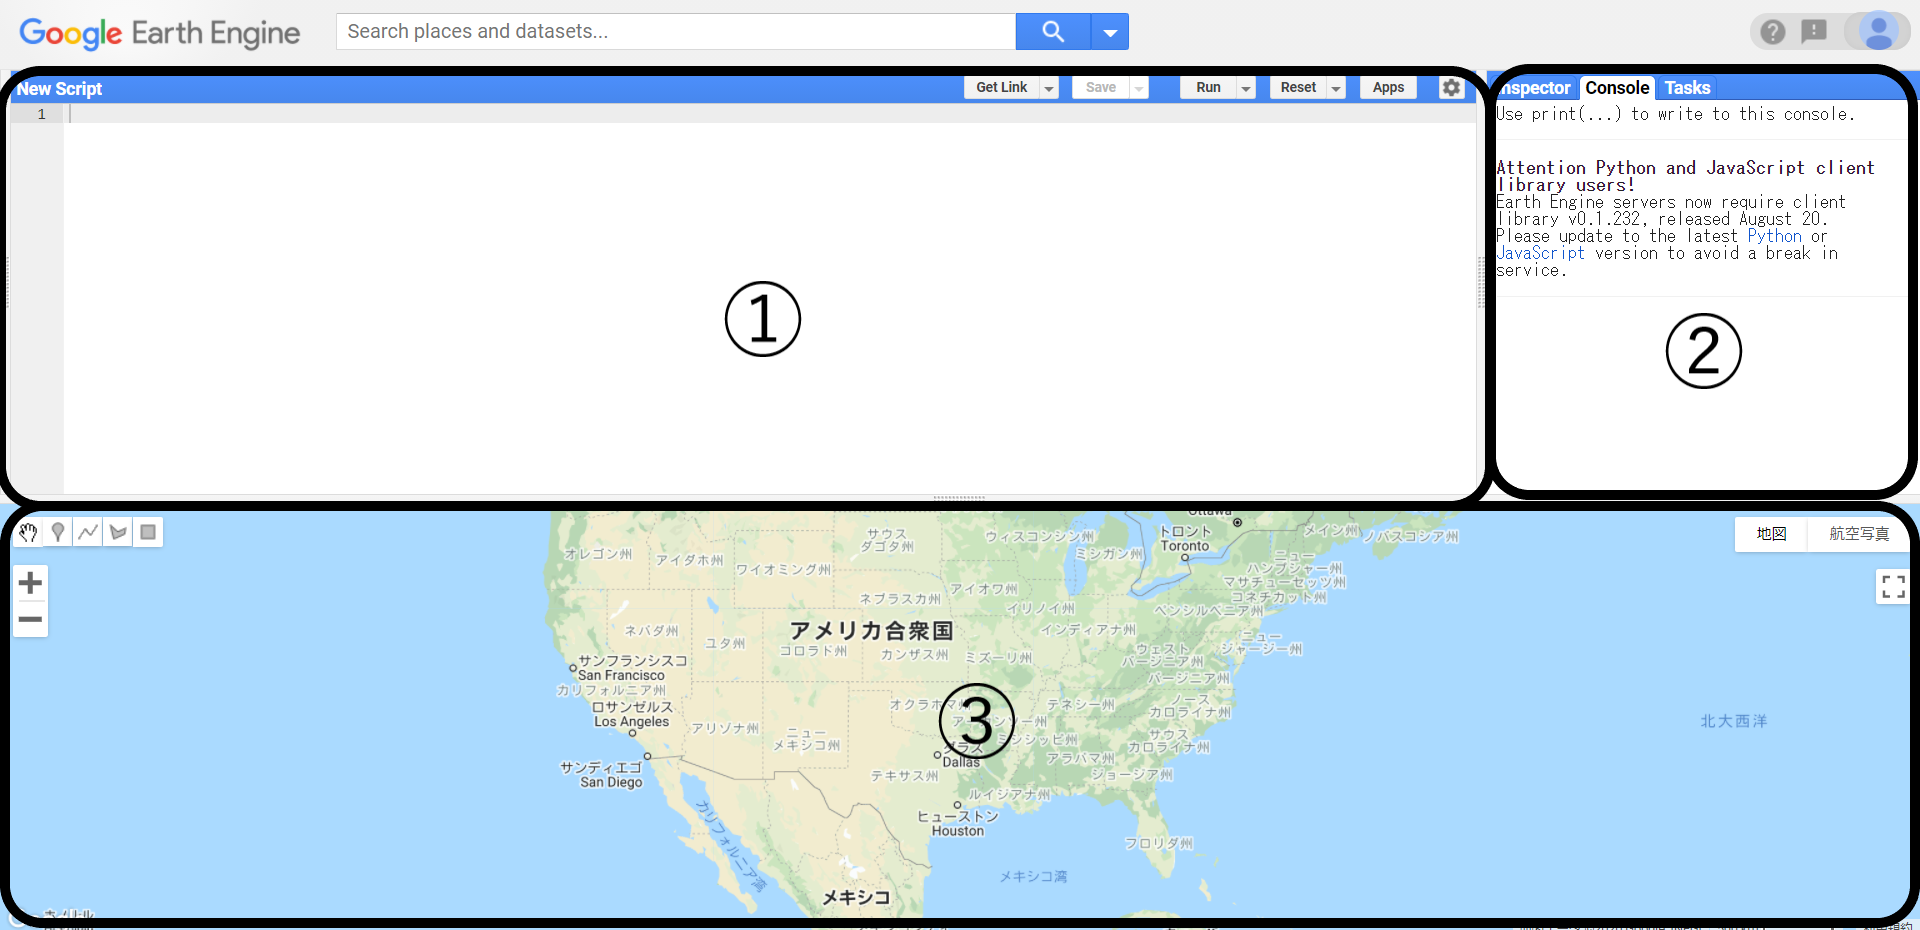
\includegraphics{images/GEE.png}
①コードの入力画面  

②  

③ 地図や結果の表示画面  

\hypertarget{gee-code-editorux3067ux6d78ux6c34ux30deux30c3ux30d7ux3092ux4f5cux6210ux3059ux308b}{%
\section{GEE code editorで浸水マップを作成する  }\label{gee-code-editorux3067ux6d78ux6c34ux30deux30c3ux30d7ux3092ux4f5cux6210ux3059ux308b}}

参考:UN Spider(\url{https://un-spider.org/advisory-support/recommended-practices/recommended-practice-google-earth-engine-flood-mapping/step-by-step})

今回の浸水マップ作成に当たっては、以下のコードを使用しました。基本的なコードは以下のURLのものと同じなので、今回は研究内容によって変更する項目について説明します。

\hypertarget{ux5bfeux8c61ux30a8ux30eaux30a2ux306eux8a2dux5b9a}{%
\subsection{対象エリアの設定}\label{ux5bfeux8c61ux30a8ux30eaux30a2ux306eux8a2dux5b9a}}

\hypertarget{ux5bfeux8c61ux65e5ux6642ux306eux8a2dux5b9a}{%
\subsection{対象日時の設定  }\label{ux5bfeux8c61ux65e5ux6642ux306eux8a2dux5b9a}}

\hypertarget{ux5404ux7a2eux8a2dux5b9a}{%
\subsection{各種設定}\label{ux5404ux7a2eux8a2dux5b9a}}

\hypertarget{final-words}{%
\chapter{Final Words}\label{final-words}}

We have finished a nice book.

  \bibliography{book.bib,packages.bib}

\end{document}
